% !TEX TS–program = pdflatexmk

\documentclass[lucida,biblatex]{sp} % use if you have the Lucida LaTeX fonts
%\documentclass{sp}          % default: uses Times font
\usepackage{textcomp}
\usepackage{graphicx}
\usepackage{algorithm}
\usepackage{algpseudocode}
\usepackage{tikz}
\usepackage{tikz-dependency}
\usepackage{gb4e}
\usepackage{amssymb}
\usepackage{pifont}
\usepackage{tipa}
\usetikzlibrary{fit,positioning}
\usepackage{setspace}
\usepackage{color}
\usepackage{bbm}
\usepackage{enumitem}
\usepackage{mathrsfs}  
\usepackage{bbm}
\usepackage{relsize}


\addbibresource{references.bib}

\usepackage[utf8]{inputenc}

%\linespread{2}


%tables
\usepackage{tabularx}
\usepackage{array}
\usepackage{booktabs}
\usepackage{multirow}
\newcolumntype{L}[1]{>{\raggedright\let\newline\\\arraybackslash\hspace{0pt}}m{#1}}
\newcolumntype{C}[1]{>{\centering\let\newline\\\arraybackslash\hspace{0pt}}m{#1}}
\newcolumntype{R}[1]{>{\raggedleft\let\newline\\\arraybackslash\hspace{0pt}}m{#1}}
\newcommand{\possessivecite}[1]{\textciteauthor{#1}'s (\textciteyear{#1})}
\renewcommand{\exp}{\text{exp }}

\newcommand{\todo}[1]{}
\renewcommand{\todo}[1]{{\bf \color{red} (TODO: {#1})}}

\newcounter{excounter}

%=====================================================================
%========================= preamble material =========================

% Metadata for the PDF output. ASCII-only!
\pdfauthor{Sebastian Schuster and Judith Degen}
\pdftitle{A Computational Model of Listener Adaptation to Speaker Variation in Use of Uncertainty Expressions}
%\pdfkeywords{Full keyword list}

% Optional short title inside square brackets, for the running headers.
% If no short title is given, no title appears in the headers.
\title{I know what you're probably going to say: \\ Listener adaptation to variable use of uncertainty expressions}

% Optional short author inside square brackets, for the running headers.
% If no short author is given, no authors print in the headers.
\author{% As many authors as you like, each separated by \AND.
  \spauthor{Sebastian Schuster and Judith Degen\\ \today}
}

%=====================================================================

\begin{document}

%=====================================================================
%============================ frontmatter ============================

\maketitle

%\begin{abstract}

%\end{abstract}

%\begin{keywords}
%  Keywords (special formatting is fine)
%\end{keywords}

%=====================================================================
%============================ article text ===========================

\section{Introduction}


% start with an example


% in one case: partner
% 60% chance of rain
% it'll probably rain
% in other case: co-worker
% 60% chance of rain
% it might rain




Imagine you are about to leave the house and your partner, who 
has read in the weather report in the local newspaper that there is a 60\% chance of a snow storm today, 
says to you: \textit{``Drive safe, there will \textbf{probably} be a snow storm today.''}

On the way to your car, you run into your neighbor, who has read the same 
weather report, and she tells you: \textit{``Drive safe, there \textbf{might} be a snow storm today.''}

As a listener, who tries to infer how likely it is that there will be a snow storm today, 
you are faced with the challenge that two different speakers described the same event probability
using uncertainty expressions that differ in strength -- \textit{probably} is conventionally a stronger
alternative to \textit{might}. In these two interactions, most contextual factors that could influence your interpretation are the same:
in both cases the Question Under Discussion \citep[QUD;][]{Roberts1996} is whether there will be a snow storm today; 
except for the uncertainty expression, the two utterances are identical and assuming that this
interaction is unrelated to the preceding conversation, the discourse context will not be helpful in 
inferring the intended event probability either.  Crucially, however, one important variable in the situation, 
namely the speaker identity, differs across these two interactions and if you have different expectations about 
how the two speakers use uncertainty expressions such as \textit{might} and \textit{probably}, 
you are more likely to infer the event probability that the speakers wanted to communicate in both situations.

As this example highlights, a listener who is faced with variability in language use 
will be able to better infer the world state that a speaker intended to communicate 
if they track individual speakers' language use and form speaker-specific expectations
about their language use. By tracking speaker-specific statistics, listeners can estimate 
accurate generative models of a speaker, i.e., models predicting what a speaker would say in different contexts, which
in return can lead to more accurate inferences of world states that specific speakers intend
to communicate.

Tracking of speaker-specific statistics and expectation adaptation has been observed in many linguistic domains, including phonetics 
\citep[e.g.,][]{Goldinger1998,Norris2003,Kraljic2005,Kraljic2007,Babel2012,Kleinschmidt2015}, 
syntax \citep{Kamide2012,Fine2013,Fine2016,Myslin2016,Kroczek2017},\footnote{Note, 
however, that some of these studies failed to replicate and it is still unclear under what 
circumstances syntactic adaptation can be observed \citep[see ][]{Liu2017,HarringtonStack2018}.} referring expressions,
\citep{Clark1986,Brennan1996,Metzing2003,Horton2005,Brennan2009}, semantics and pragmatics \citep{Yildirim2016, Wittenberg2016}, 
lexical associations \citep{DelaneyBusch2019},
and intonation and prosody \citep{Kurumada2012,Roettger2019}. 

At most linguistic levels, it also
seems clear what kind of expectations listeners are updating. At the level of phonetics, for example, 
listeners seem to be updating their expectations about speakers' \textbf{associations} between acoustic cues and phonemes \citep[e.g.,][]{Kleinschmidt2015}.
At the level of syntax, listeners seem to be updating expectations about speakers' \textbf{preferences} 
for different syntactic structures.  At the level of semantics, however, the adaptation processes are still poorly understood.
In particular, while the results by \cite{Yildirim2016} suggest that listeners are updating 
\textit{some} expectations about specific speakers' language use, 
it is an open question what kind of expectation updates underlie semantic/pragmatic adaptation. 
Answering this question is the focus of the current study.

Conceptually, from a Gricean perspective of utterance interpretation \citep{Grice1975}, 
there seem to be two likely types of expectations that could get updated during semantic/pragmatic adaptation.
It could be that, analogously to phonetic adaptation, listeners are tracking speakers' associations between 
words and world states, i.e., the speakers' lexica. It could also be that, analogously to syntactic adaptation, 
listeners are tracking speakers' preferences
for different words. Further, it could also be that listeners are tracking both associations and preferences.

To illustrate how different beliefs about lexica and utterance preferences can lead to different interpretations, consider the interpretation 
of the uncertainty expression \textit{probably} produced by different speakers. For the sake of this example, 
let us assume the only three expressions that a speaker can choose from are \textit{might}, \textit{probably}, and \textit{almost certainly}.
A listener's beliefs about the three speakers' lexica and preferences are schematically illustrated in Figure~\ref{fig:inference-example}.

First, consider speaker {\bf A}, for whom \textit{might} is semantically felicitous if the event probability exceeds 10\%, 
\textit{probably} if the event probability exceeds 60\% and \textit{almost certainly}  if the event probability exceeds 90\%. 
If a listener has accurate beliefs about {\bf A}'s mapping between utterances and event probabilities, they will be likely to infer an event probability
between 60 and 90\% when they hear {\bf A} produce \textit{probably}.

Now, consider speaker {\bf B}, for whom \textit{might} is semantically felicitous if the event probability exceeds 30\%, 
\textit{probably} if the event probability exceeds 75\% and \textit{almost certainly}  if the event probability exceeds 95\%. If a listener has
accurate beliefs about {\bf B}'s mappings, they will be likely to infer an event probability between 75\% and 95\% when they hear {\bf B} produce 
\textit{probably}.

Lastly, consider speaker {\bf C}. {\bf C} uses the same mapping between utterances and event probabilities as {\bf B}. However, {\bf C} very rarely
produces \textit{almost certainly}. If a listener has accurate beliefs about {\bf C}'s mappings and {\bf C}'s utterance preferences, 
they will be likely to infer an event probability between 75\% and 100\% when they hear {\bf B} produce \textit{probably} since they will not
consider  \textit{almost certainly} a likely alternative and will therefore be less likely to draw a scalar inference \citep[e.g.,][]{Horn1984}. 







%mention connection to pickering \& garrod

%mention connnection to horton \& gerrig





%for lower-level processing, we also know what kind of statistics listeners keep track of: 



%To what extent and how we learn such speaker-specific expectations is still poorly understood.
%\citet{Clark1986} were among the first to study how listeners learn speaker-specific 
%referring expressions for abstract figures. They found that despite large variability in how speakers 
%initially refer to these abstract figures, a pair of interlocutors quickly formed \textit{conceptual pacts} for referring expressions  
%in a collaborative director-matcher task.  Similarly, \citet{Brennan1996} found that interlocutors kept 
%referring to cards with objects using referring expressions 
%that are more specific than necessary in context if they previously had used the more
%specific expression in the conversation.

%More generally, speaker variation exists and corresponding listener adaptation 
%happens at many, if not all, linguistic levels. At the level of phonetics 
%listeners rapidly update their beliefs about a specific speaker's phoneme boundaries after 
%listening to the speaker produce words for a short period of time (e.g., \cite{Norris2003,Kraljic2005,Kraljic2007}). 
%This suggests that listeners form speaker-specific mappings from acoustic cues to phonemes when listening to a speaker.
%At the level of syntax, listeners mirror speakers' attachment preferences of temporally ambiguous relative clauses 
%after a brief exposure to specific speakers \citep{Kamide2012}. 
%Similarly, \cite{Kroczek2017} found that listeners differ in their interpretation of 
%German sentences with a word order ambiguous between SVO and OSV, 
%depending on the proportion of OSV sentences produced 
%by the speaker during an exposure phase.
%In self-paced reading experiments, garden-path effects disappear in sentences with reduced 
%relative clauses over the course of the experiment, which suggests that 
%readers update their beliefs about the writer's distribution of syntactic constructions 
%during the experiment \citep{Fine2013,Fine2016}. 
%Further, \citet{Yildirim2016} showed 
%that adaptation is not limited to lower-level language processing. In their experiments, 
%listeners form speaker-specific expectations regarding the use of the quantifiers \textit{some}
%and \textit{many}. Specifically, they exposed participants to short video clips of a speaker describing 
%a bowl which contained blue and green candies. In the critical exposure trials, the speaker consistently
%described situations in which there were approximately equal numbers of blue and green candies either with 
%\textit{``Some of the candies are green''} (\textit{some-biased} condition) or with \textit{``Many of the candies are green''}
%(\textit{many-biased} condition). They found that participants in the \textit{some-biased} condition on average thought that 
%the speaker was more likely to use \textit{some} to describe candy bowls for a larger range of green candy proportions than in the 
%\textit{might-biased} condition. These results also hold when participants are exposed to two speakers, one some-biased speaker
%and one many-biased speaker. After the exposure phase, participants thought that the some-biased speaker was more likely to use \textit{some} 
%for a larger range of green candy proportions and that the many-biased speaker was more likely to use \textit{many} for a larger 
%range of green candy proportions. Based on these results, \citet{Yildirim2016} argued that listeners keep track of how specific speakers
%use quantifiers and form speaker-specific expectations of language use. 

%The conclusion drawn in all these studies is that listeners update their beliefs about specific speakers' language use to facilitate
%rapid language comprehension. For several domains, this qualitative prediction has been formalized using computational models
%to make quantitative predictions of listeners' behavior after being exposed to specific speakers or writers. \cite{vanSchijndel2018} propose
%a connectionist model based on a dynamic neural language model whose weights are updated after processing each sentence.
%They showed that their model's predicted surprisal strongly correlates with participants' reading times in the experiment by \cite{Fine2016}.
%At the same time, computational models based on Bayesian belief updating were shown to accurately predict post-adaptation behavior
%for several domains. \cite{Kleinschmidt2015} introduced a computational model to predict listeners' phoneme categorization behavior 
%after exposure to different speakers. They assume that
%listeners have speaker-specific distributions from acoustic cues to phonemes and that the update of these distributions in interaction
%can be modeled as Bayesian belief updates. \cite{Fine2010} also presented a Bayesian model in which they assume that listeners
%update their beliefs about a speaker's distribution over different syntactic structure. Further, \cite{DelaneyBusch2019} presented a 
%Bayesian model of adaptation in semantic priming experiments. 
%Based on their modeling experiments, they argued that participants adapt to the rate of semantically similar words in a given context 
%which in return affects the size of a N400 effect in response to a semantically unrelated word. Lastly, \cite{Roettger2019} presented a Bayesian belief
%updating model
%of adaptation to variable use of intonational cues and \cite{Hawkins2017} presented a Bayesian model of the formation of conceptual pacts.
%In short, there is a growing body of evidence that linguistic adaptation can be seen as an instance of Bayesian belief updating of
%expectations about language use, which potentially suggests that such a process is a general linguistic mechanism operating at all linguistic levels.

%Following this line of work, we investigate whether semantic adaptation effects as observed by \cite{Yildirim2016} can be explained by similar 
%Bayesian belief updating processes, and what kind of expectations listeners update when adapting to a speaker. Analogous to syntactic adaptation, it 
%could be that semantic adaptation is a result of listeners forming speaker-specific expectations about lexical preferences, i.e., 
%listeners learn in interaction that a speaker prefers certain expressions over others. Analogous to phonetic adaptation, it could also 
%be that listeners are forming speaker-specific expectations about lexica, i.e., listeners learn speaker-specific form-meaning mappings. 
%Further, it could be that semantic adaptation is a result of listeners updating expectations about preferences and lexica.

In this work, we investigate the nature of semantic adaptation through a combination of experiments and computational modeling.
We study this phenomenon in the domain of uncertainty expressions. 
We define uncertainty expressions as words or phrases that can be used to express uncertainty about 
whether a future event will happen or not. This includes epistemic modals (see, for example, \citep{Kratzer1991} and \citep{Hacquard2011}) such as \textit{might}, 
\textit{probably}, and \textit{could} but also phrases such as \textit{it looks like} which were primarily investigated by the experimental literature (e.g., \cite{Kurumada2014,Pogue2018}).
Uncertainty expressions have several properties that make them a good testing ground for studying semantic and pragmatic
adaptation. First, there is no direct mapping between uncertainty expressions and a speaker's belief about the likelihood of future events 
(see, for example, \citet{Clark1990}, \citet{PepperPrytulak1974}). Second, there is considerable inter-speaker variability 
in the use of these expressions \citep{Wallsten1986} and therefore it is likely that listeners expect different speakers to use these expressions
differently. Lastly, interpreting uncertainty expressions play an important role in many everyday situations such as communicating and  
interpreting health risks \citep{Berry2004, Lipkus2007, Politi2007} or making financial decisions \citep{Doupnik2003}. 
For this reason, listeners often have a vested interest in inferring  how a given speaker uses these expressions and are therefore 
potentially more attuned to subtle differences across speakers than in cases where variation tends to have less of an effect on making decisions.

The rest of this paper is structured as follows. In the next section, we present results from a norming study that show that listeners vary in their
expectations of what uncertainty expressions a generic speaker will use to describe different event probabilities. 
In section~3, we present a game-theoretical computational model of listeners expectations about a generic speaker's use of uncertainty expressions.
In section~4, we present an experiment that provides evidence for listener's updating their expectations after brief exposure to different speakers.
In section~5, we present our adaptation model and argue based on model simulations that listeners are updating their expectations about preferences and
lexica.
In section~6, we discuss how our model also predicts updated interpretations of uncertainty expressions after a brief exposure to a different speaker and 
we present an experiment whose results confirm this prediction. We conclude this paper with a discussion of remaining open questions and the implications of our findings.

\section{Pre-exposure ratings}

We first conducted a series of norming studies, which served the following purposes.
First, they allowed us to investigate whether listeners vary in their expectations about
a generic speaker's use of uncertainty expressions in our experimental context. 
Second, they served as a check whether our paradigm and the manipulation of different event probabilities work. 
Third, we used the results from these studies to inform the experimental design of the adaptation experiments. 
Lastly, as we will discuss in Section 5, we used the data collected in the norming studies to 
estimate population-level prior beliefs for our adaptation model.

\subsection{Participants}
We recruited a total of 420 participants 
(20 per condition) on Amazon Mechanical Turk. 
We required participants to have a US-based IP address and a minimal approval rating of 95\%.
Participants were paid \$1.80 (condition 1), \$1.50 (conditions 2-15),
or \$2.00 (conditions 16-21),
%; condition 6a), 
depending on the number of trials,
which amounted to an hourly wage of approximately \$12--\$15. 

\begin{figure}
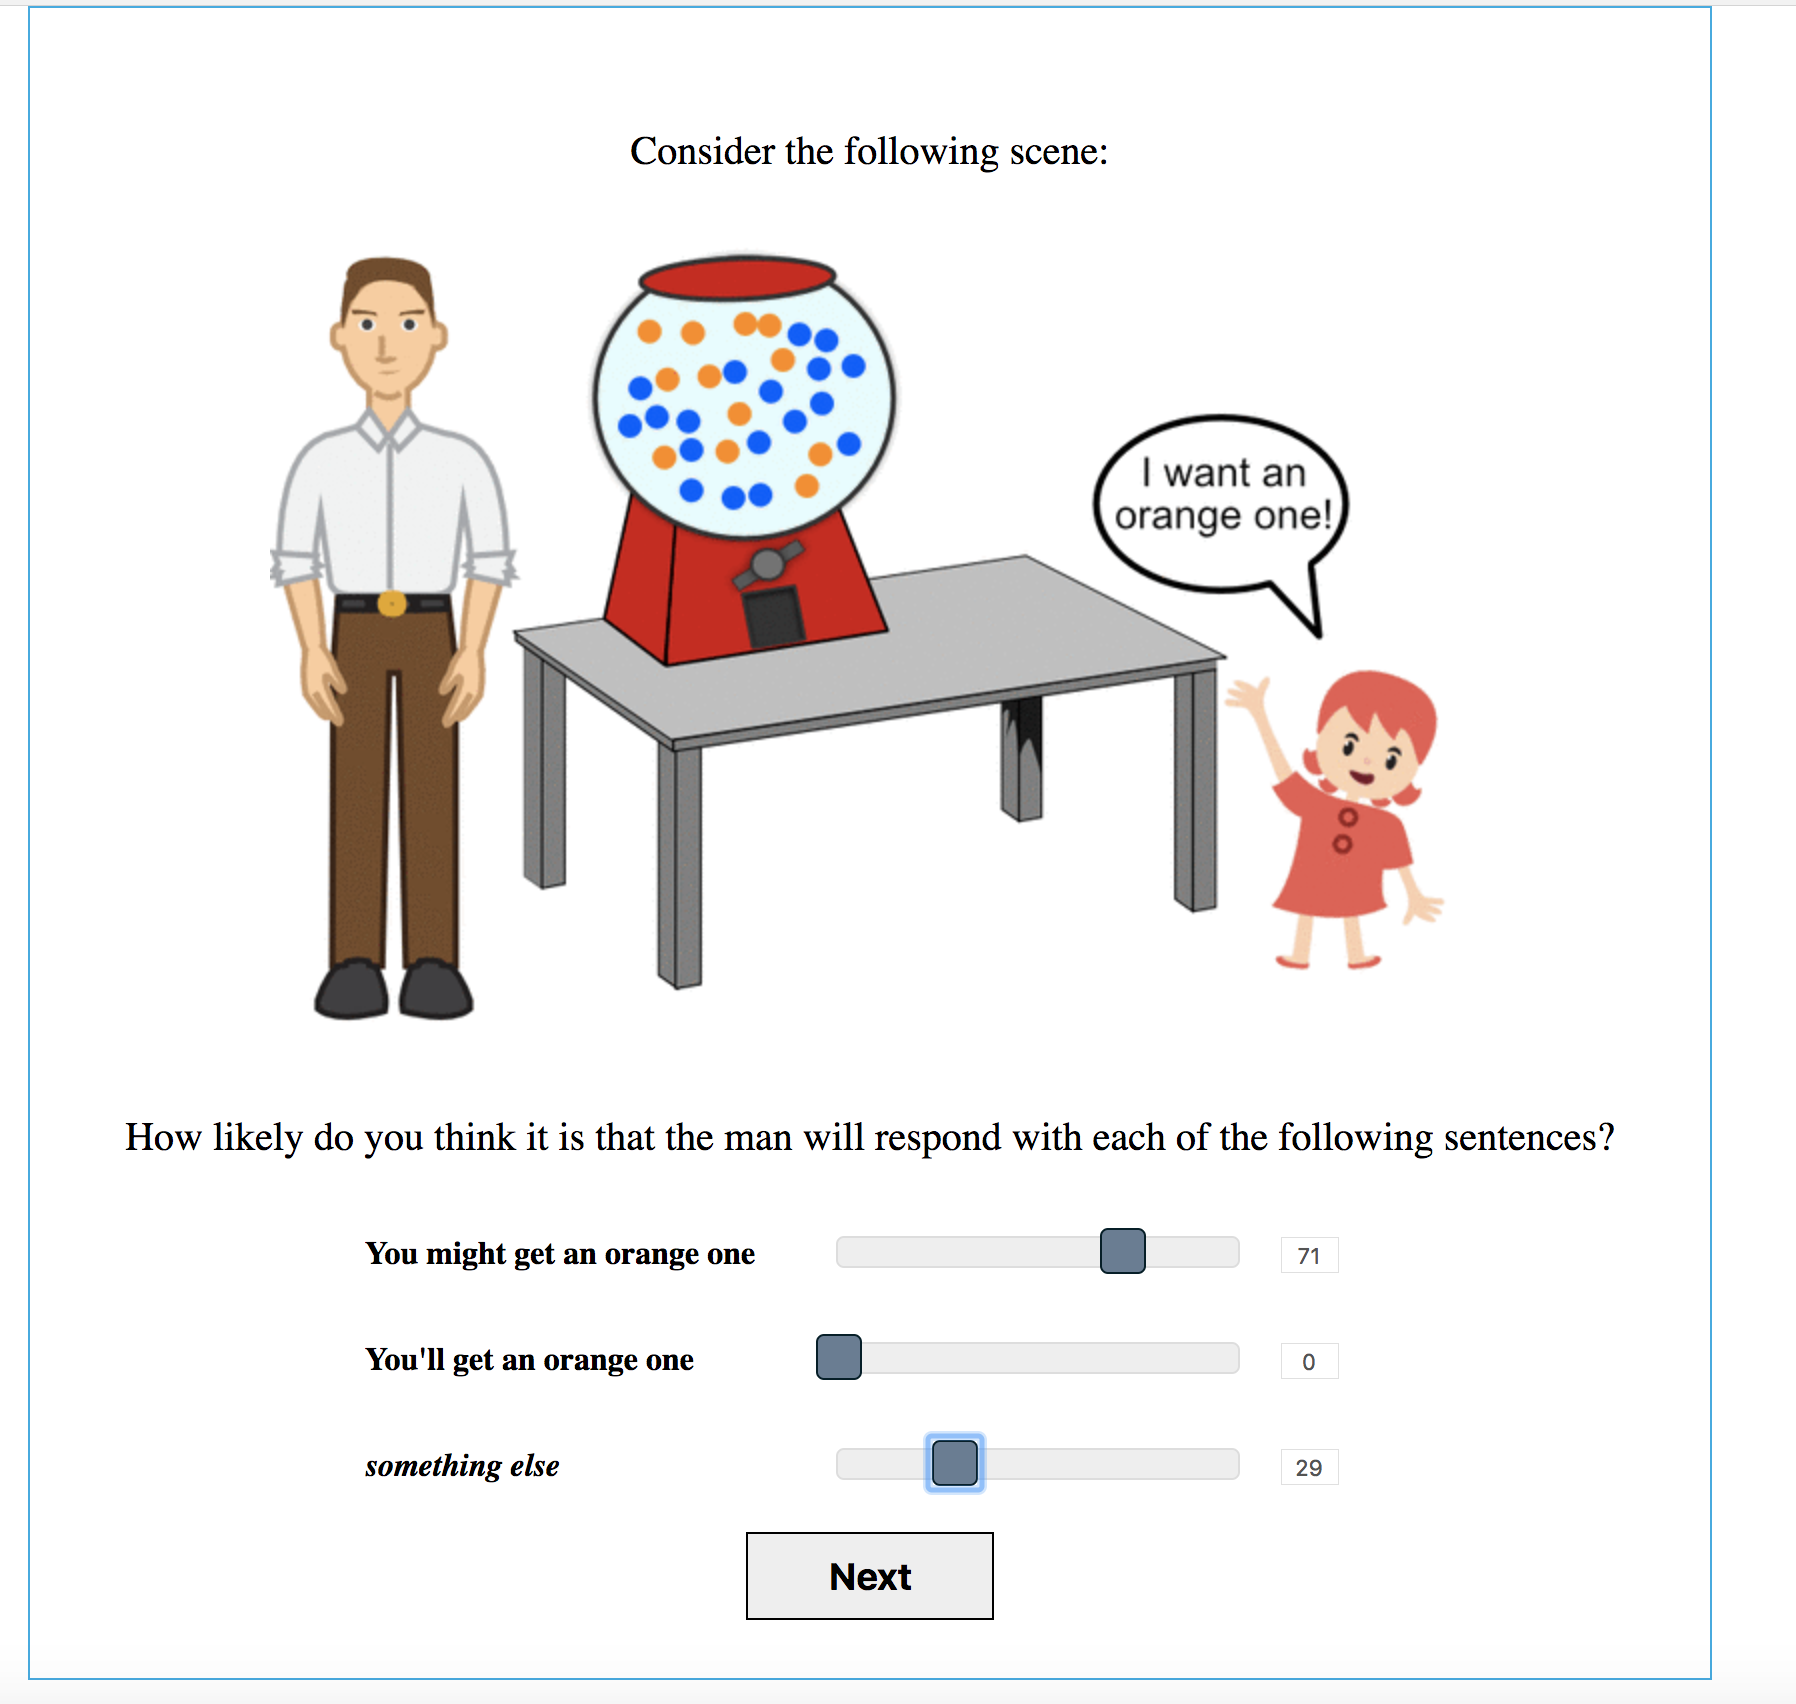
\includegraphics[width=\textwidth, trim={0 0 1.1cm 0},clip]{plots/pre-test-example-trial.png} 
\caption{Example trial from norming study. \label{fig:norming-trial} }
\end{figure}

\subsection{Materials and Procedure}
The norming study was a forced-choice production experiment. Participants were instructed 
that over the course of the experiment, they would see several scenes with an adult man, 
a young girl, and a gumball machine on a table and 
that the gumball machine is too high up on the table for the girl to see. 
After completing an attention check which asked participants whether 
the girl could see the gumball machine,\footnote{Participants had to go back to the instructions in case they responded incorrectly. This was the case for 41 participants.} 
participants saw a series of scenes (see Figure~\ref{fig:norming-trial} for an example scene) and were asked to rate how likely they thought it was that the 
adult would produce two given responses by distributing 100 points across the two given utterances and the 
blanket \textit{something else} option. Sliders automatically jumped back if participants tried to distribute more than 100 points. 
In each scene, the child uttered \textit{``I want a blue one''} (target color: blue) or  \textit{``I want an orange one''} (target color: orange)
(randomized across participants\footnote{In condition 1 (\textit{bare-might}), as well as conditions 16-21 (all conditions with \textit{bare not}), the target color was randomized across trials. While randomization of the target color across trials increased the correlation between the ratings for the two colors,  the average ratings for each condition independent of the target color were not affected by this choice. See the supplementary material for a detailed discussion of the effect of this manipulation on the ratings.}). The gumballs in the machines were being tossed around to prevent participants counting the gumballs
and to make sure that participants did not consider it more likely to get one of the gumballs at the bottom of the machine.
 In each of the 21 conditions, participants saw only  two of the following seven possible adult utterances with different uncertainty expressions:

 \begin{itemize}
\item You'll get a blue/orange one (\textsc{bare})
\item You might get a blue/orange one (\textsc{might})
\item You'll probably get a blue/orange one (\textsc{probably})
\item I think you'll get a blue/orange one (\textsc{think})
\item It looks like you'll get a blue/orange one (\textsc{looks like})
\item You could get a blue/orange one (\textsc{could})
\item You won't get a blue/orange one (\textsc{bare not})
\end{itemize}


\noindent Within each condition, we manipulated the percentage of target color gumballs across trials. 
Each participant saw 3 trials\footnote{In condition 1 (\textit{bare-might}), participants saw each gumball machine 6 times -- 3 times when being asked to produce a statement about orange gumballs and 3 times when being asked to produce a statement about blue gumballs. In conditions 15-20 (all conditions with \textit{bare not}), participants saw each machine 4 times: 2 times for each color.} 
for each of the following percentages: \\ 0\%, 10\%, 25\%, 40\%, 50\%, 60\%, 75\%, 90\%, 100\%.

\noindent We randomized the order of expressions across participants and trials were presented in pseudo-randomized order.


\subsubsection{Results and Discussion}

\begin{figure}
\includegraphics[width=\textwidth]{plots/pre\string_test\string_main.pdf} 
\caption{Results from 3 conditions of the norming study. Error bars correspond to bootstrapped 95\%-confidence intervals. \label{fig:norming-results-main} }
\end{figure}

Figure~\ref{fig:norming-results-main} shows participants' ratings for different gumball proportions for 3 of the 21 conditions, namely all combinations of the conditions
with the utterances \textsc{bare}, \textsc{probably}, and \textsc{might}. 
(see the Supplementary Material for the results from other conditions). 
The results from these three conditions highlight several important properties about participants'
behavior in this experiment that generalize to all conditions.
First, the ratings for individual utterances are influenced by the utterance choices presented to participants.
If we compare the ratings for \textsc{might} in the \textit{bare-might} and the \textit{might-probably} condition, we see that \textit{might} received high ratings for a larger
range of event probabilities when it is paired with \textsc{bare} than when it is paired with \textsc{probably}. We observe similar effects for the other two utterances.
This suggests that participants are primed to use the utterances provided in the experiment and that their ratings depend on the presented alternatives -- an effect that
has also been observed for quantifiers \citep{DegenTanenhaus2015}.

Second, the results suggest that participants are sensitive to the different event probabilities and that our paradigm is well suited to study 
the mapping between event probabilities and uncertainty expressions. For example, in the \textit{might-probably} condition, participants
provided considerably different ratings when they were presented with a gumball machine with 50\% target color gumballs than when they
were presented with 60\% target color gumballs.

\begin{figure}
\includegraphics[width=\textwidth]{plots/pre\string_test\string_main\string_indiv.pdf}
\caption{Results of three individual participants in the \emph{might-probably} condition of the norming study. \label{fig:norming-results-indiv}}
\end{figure}


Third, in all conditions, the mean ratings are graded and except for the 0\% and 100\% target color gumball trials, the average rating for none of the
utterances is close to 100. There are two potential explanations for this observation. It could be that participants provided categorical ratings, i.e.,
generally assigned 100 points to one of the three options but the category boundaries vary across participants which leads to the graded average ratings.
It could also be that participants' individual ratings are graded which could reflect participants' uncertainty about which utterance a speaker would use 
and that these individual graded ratings drive the  graded average ratings. If we look at individual participants' ratings, it appears to be a combination of both.
Figure~\ref{fig:norming-results-indiv} shows the responses of three individual participants in the \emph{might-probably} condition. These figures show that there 
is a range of gumball proportions for each participant for which they assigned similar ratings to two utterances, which suggests uncertainty about the speaker's 
utterance choice. At the same time, however, this range also differed across participants: Participant \#8, a ``\textit{cautious}'' speaker, thought that the speaker would only be likely to use {\sc probably} 
when the objective probability of getting a target color gumball was greater than 75\%, whereas participant \#15, a ``\textit{confident}'' speaker, thought that  {\sc probably} was a better utterance choice than {\sc might} 
when the objective probability of getting a target color gumball was just greater than 50\%. These observations suggest that participants have uncertainty about a 
speaker's use of uncertainty expressions and that they have a priori different expectations about how a generic speaker would use these expressions.

This uncertainty and variability seems to be particularly borne out in the \emph{might-probably} condition. For this reason, we chose this pair of expressions
to study listeners' adaptation to variable uses of uncertainty expressions.


\section{Production belief model}

The norming data confirmed previous findings that participants' expectations 
about how a generic speaker would use uncertainty expressions 
depend on the set of utterances that participants can choose from.
We further found that ratings were graded since participants seemed to have uncertainty
in their expectations about how a generic speaker would use uncertainty expressions.
Hence, a model predicting participants' beliefs about a speaker's productions of uncertainty expressions
 should  (a) be able to capture differences based on the availability of alternative utterances; 
(b) provide graded predictions; 
and (c) be able to capture uncertainty within participants.

Computational game-theoretic models such as the Rational Speech Act (RSA; \cite{Goodman2016}) 
framework are uniquely suited to fulfill these desiderata.
Crucially, RSA models  base their predictions on a set of alternative utterances and 
they make probabilistic predictions.  According to an RSA model, a speaker who wants to
 convey some information to a listener 
chooses her utterance based on the utterance utility compared to the utility of alternative utterances. 
The speaker's utility of an utterance is determined by taking the listener utility and the speaker cost into accounnt: 
it is the difference between the informativity of the utterance to a listener and the speaker's cost of the utterance.

In defining the informativity of an utterance, we follow previous RSA models of uncertainty expressions (\cite{Lassiter2013,Herbstritt2019}) 
and assume that uncertainty expressions have a threshold semantics, 
i.e., for each uncertainty expression $u$, there exists some threshold $\theta_u \in [0,1]$ 
such that an utterance with $u$ is semantically felicitous if the probability $\phi$ 
of the proposition embedded under $u$ exceeds $\theta_u$. 
For example, if we assume the threshold for \textit{might}, $\theta_{might}$, is 0.1, then the statement 
``It might rain this afternoon'' is true if the probability of rain in the afternoon exceeds $0.1$. 
Formally, we base the computation of informativity on a probability distribution from utterances to event probabilities $\phi$, 
which is usually referred to as the \textit{literal listener} $L_0$ in the RSA framework. 

$$L_0\left(\phi \mid u, \theta_u\right) \propto P(\phi) 1\left[\phi > \theta_u \right] \qquad \mbox{(for positive utterances)}$$
$$L_0\left(\phi \mid u, \theta_u\right) \propto P(\phi) 1\left[\phi < \theta_u \right] \qquad \mbox{(for negated utterances)}$$

$P(\phi)$ is a prior distribution over event probabilities, which is independent of the utterance by the speaker.


A \textit{pragmatic speaker} $S_1$ who wants to communicate an event probability $\phi$ then chooses her utterance $u$ from a set of utterances $U$ according to a soft-max choice rule \cite{Luce1959,SuttonBarto} such that she chooses $u$ with a probability proportional to her speaker utility. 
$$S_1\left(u \mid \phi, \theta, c\right) \propto \exp \left( \lambda \left( \log L_0\left(\phi \mid u, \theta_u\right)  - c(u)\right)\right)$$
$\lambda$ is a rationality parameter which governs how likely a speaker is to choose the utterance that maximizes her utility; as $\lambda$ approaches infinity, a speaker is more likely to always choose the optimal utterance.  


\begin{figure}
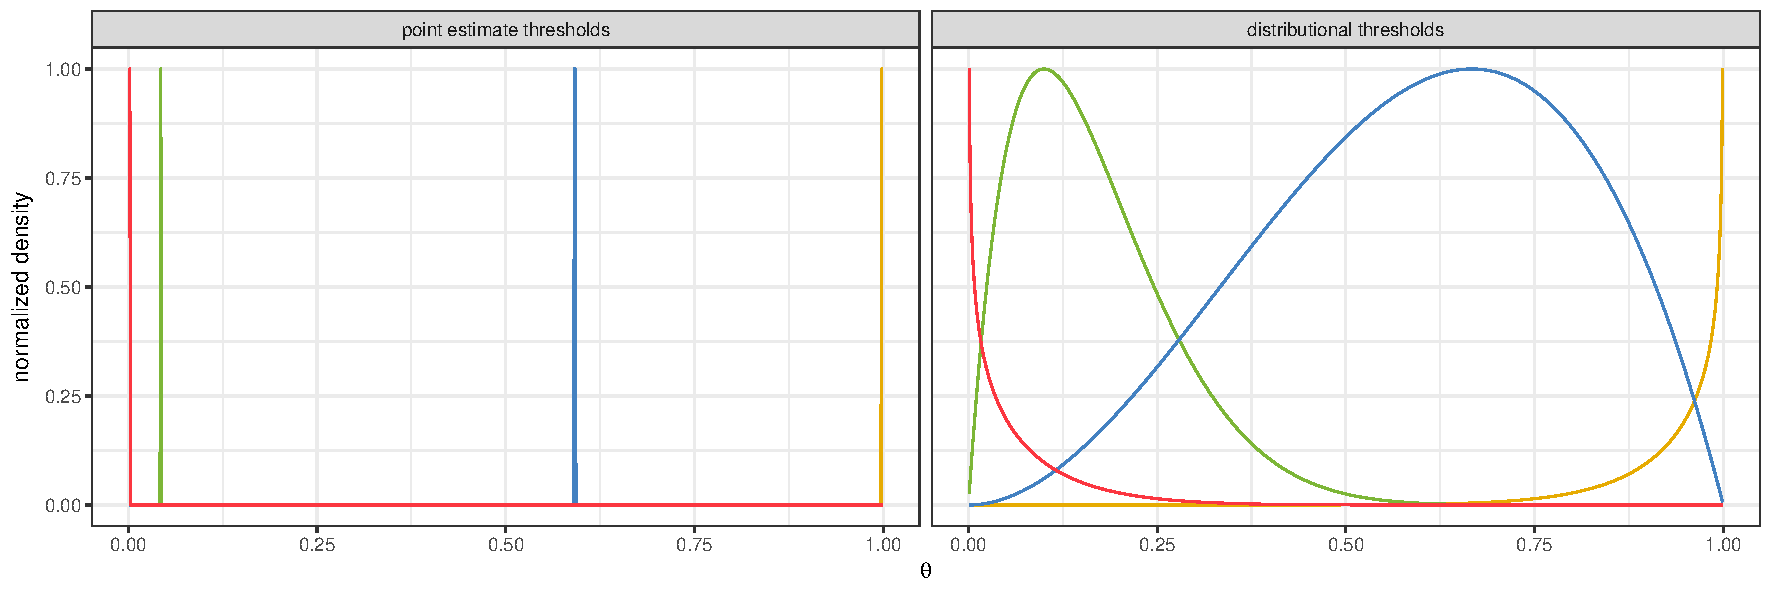
\includegraphics[width=\textwidth]{plots/model-visualization-distributions.pdf}

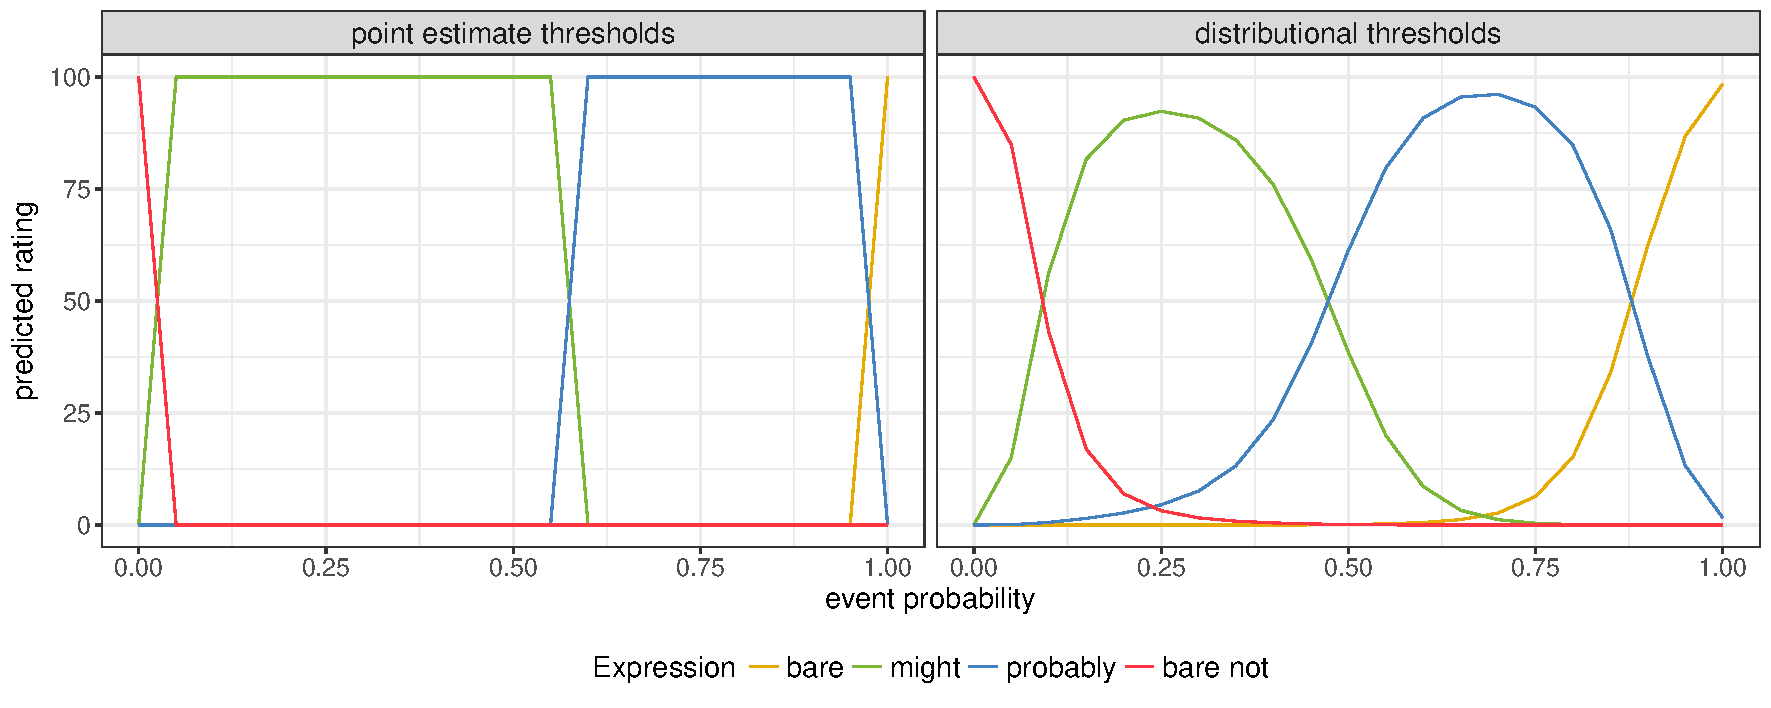
\includegraphics[width=\textwidth]{plots/model-visualization-predictions.pdf}

\caption{Example threshold distributions (upper panels) and corresponding model predictions by the \textit{expected pragmatic speaker} model (lower panels). In this example, the set of possible utterances is $U=\{$\textsc{bare}, \textsc{might}, \textsc{probably}, \textsc{bare not}$\}$, all utterances have equal costs, the rationality parameter $\lambda$ is set to 10, and the prior probability over event probabilities $P(\phi)$ is a uniform distribution. As the panels on the left show, point estimates of thresholds lead to sharp categorical boundaries in the model predictions, whereas distributions over thresholds, as in the panels on the right, lead to gradually increasing and decreasing predicted utterance ratings. \label{fig:model-visualization}}
\end{figure}



$S_1$ crucially depends on a vector of thresholds $\theta$ which contains a threshold for each utterance in $U$, 
as well as  a cost function $c(u)$, and it is still largely an open question what values speakers and listeners assign 
to these variables. In our norming studies, we found that both at the population-level and at the individual-level, 
participants' ratings of the different expressions gradually increased and decreased with changing event probabilities 
(as, for example, shown in Figure~\ref{fig:norming-results-indiv}). This is expected if we assume that participants
have probabilistic beliefs about thresholds $\theta$ (as illustrated in the right panels of Figure~\ref{fig:model-visualization}) but not so if we assume that
participants are reasoning based on point estimates of $\theta$ (as illustrated in the left panels of Figure~\ref{fig:model-visualization}).
Considering these observations,  we assume that listeners hold beliefs about speakers' thresholds  in the form of a distribution $P\left(\theta_u\right)$.\footnote{We leave it open 
whether a speaker samples from a distribution over thresholds when making utterances (as suggested by \citet{Qing2015}) 
or always uses the same values for thresholds. In the former case, listeners could have higher-order beliefs  $P(\eta)$ 
about different speakers' threshold distributions instead of having direct beliefs about the thresholds that different 
speakers use. For our purposes, this distinction does not matter since we would assume that listeners marginalize over their higher-order beliefs $P(\eta)$ such that  $P\left(\theta_u\right) = \int P\left(\eta\right) P\left(\theta_u \mid \eta\right) d\eta$ and we therefore take the simplest approach and directly model $P\left(\theta_u\right)$. } Analogously, we assume that listeners also have beliefs $P(c)$ about the speaker's cost function.
Using these two distributions, we can define the \textit{expected pragmatic speaker} $ES_1\left(u \mid \phi \right)$ as follows:

$$ES_1\left(u \mid \phi \right) = \int P(c) \int_0^1 P(\theta) S_1\left(u \mid \phi, \theta, c\right) d\theta \  d c$$

This model predicts what a listener having uncertainty about a speaker's thresholds (or threshold distributions) and cost function would expect that speaker to say in different situations.
Intuitively, this model is a weighted average of different speaker models with differing thresholds and cost functions where the weights are determined by the listener's belief distributions over thresholds
and costs. 

%$P(\theta)$ serves two purposes here: On the one hand, it captures the variability in expectations across participants and on the other hand, it captures individual participants' uncertainty. 
%In theory one could separate these two distributions by having one distribution modeling the variability across participants and then having a separate distribution for each listener capturing
%their uncertainty. Since we are primarily concerned with modeling population-level expectations in this work, we decided to conflate these two source of variability.


%\textbf{TODO:} walk through example model and show how this model is capable of pragmatic inferences and different preferences

\subsection{Linking function}

Overall, we assume that participants' reason about what they believe a speaker would say 
in different situations when asked to provide ratings for utterances. 
We assume that these beliefs are guided by participants' beliefs about the speaker's thresholds and costs, and 
that participants are averaging over their uncertainty. For this reason, we assume that the population-level 
average ratings of what participants expect the speaker to say in different situations 
correspond to the probabilities predicted by the \textit{expected pragmatic speaker} model.
However, given the forced choice nature of the experiment and that we are estimating model parameters from limited and potentially noisy data, we make the following additional linking assumptions.

\begin{itemize}
\item \textbf{Set of utterances}: Across all conditions, we assume that the set of utterances that participants are considering is the set of all utterances that we used in the norming study, i.e., $U= \{$ \textsc{bare}, \textsc{might}, \textsc{probably}, \textsc{think}, \textsc{looks like}, \textsc{could}, \textsc{bare not}$\}$. We include all utterances instead of only the utterances that are presented in a given condition since we assume that participants' general knowledge about English uncertainty expressions also influences their ratings. Ideally, we would include even more utterances in this set of alternatives but since we can only estimate parameters for uncertainty expressions for which we collected ratings, we are limited to the expressions in $U$.

\item \textbf{\textit{something else} option}: Participants in condition $\mathscr{C} = \{u_a, u_b\}$ 
could only choose between the three utterances $U' = \{u_a, u_b,$ \textit{something else}$\}$.
For modeling data from condition $\mathscr{C}$, we therefore need a function to predict the ratings 
for the utterances in $U'$. For $u_a$ and $u_b$, this is straightforward: We assume the probability 
of a participant choosing $u_a$ or $u_b$
is proportional to $ES_1(u_a \mid \phi)$ and $ES_1(u_b \mid \phi)$, respectively. 
We model the probability of a participant choosing the \textit{something else} option as the sum 
of the probability of all utterances that were not part of the condition as well as a constant $O$, 
which accounts for probability mass assigned to utterances that participants might be 
considering but which are not contained in $U$. This gives us the following condition-specific 
function $ES_1^{(\mathscr{C})}$ for predicting participants' ratings.

$$
ES_1^{(\mathscr{C})}(u \mid \phi) \propto 
     \begin{cases}
       ES_1(u \mid \phi) &\quad\text{if } u  \in \mathscr{C}\\
       O + \sum_{u \not \in \mathscr{C}} ES_1(u \mid \phi) &\quad \mbox{if $u$ is \textit{something else}} \\
     \end{cases}
$$

\item \textbf{Cost function}: We assume that the cost function represents participants' beliefs about the speaker's 
preferences for different utterances. Lower costs of an utterance indicate higher speaker preferences. We further 
assume that we are cueing participants to believe that the speaker would be likely to use the two utterances, $u_a$ 
and $u_b$, that are provided in condition $\mathscr{C}=\{u_a, u_b\}$ and that participants therefore primarily use the 
\textit{something else} option when both of the two utterances are semantically infelicitous or otherwise highly unexpected. 
We model this cueing effect in our choice of the cost function $c(u)$, which depends on the condition. For the two utterances 
that are presented to the participants, we set the cost to $1$ and for all the other utterances, we set the cost to a constant $\gamma$:
$$
c(u, \mathscr{C}) = 
     \begin{cases}
       1 &\quad\text{if } u  \in \mathscr{C}\\
       \gamma &\quad\text{otherwise} \\
     \end{cases}
$$

Theoretically, we could have also used a different constant $\gamma_u$ for each utterance. The data from
the norming experiments, however, suggests that participants generally did not prefer one utterance over 
the other. To limit the number of free model parameters and to prevent overfitting, we therefore use a single
constant $\gamma$ for all utterances. 

\item \textbf{Noise}: Finally, to account for participants not paying attention or making mistakes, 
we also include a noise term that models participants providing random ratings.
The amount of noise is captured by the noise strength parameter $\delta$. This parameter
indicates the proportion of random responses, that is, the proportion of responses drawn from a uniform distribution
over the three condition-specific responses $U'$. 

\end{itemize}

\noindent Incorporating all of these assumptions, we end up with the following noisy, condition-specific expected pragmatic speaker 
model $ES_1^{(\mathscr{C})'}(u \mid \phi)$, which we use to predict participants' ratings:

$$ES_1^{(\mathscr{C})'}(u \mid \phi) = \delta \times \frac{1}{|U'|} +  (1 - \delta) \times ES_1^{(\mathscr{C})}(u \mid \phi)$$

For the prior distribution over event probabilities $P(\phi)$, which is used in the literal listener $L_0$, 
we use a uniform distribution over the interval $[0,1]$.\footnote{To 
verify the assumption that the prior on event probabilities is uniform, we conducted a separate norming study in which participants rated 
how likely they thought it was that a speaker described different gumball machines containing different 
proportions of blue and orange gumballs after hearing an unintelligible utterance. We found that on average 
participants rated all gumball machines equally likely which suggests that the prior over event probabilities is 
indeed uniform.} For the distributions over thresholds $P(\theta_u)$, we use a Beta distribution parametrized by 
$\alpha_u$ and $\beta_u$. The choice of Beta distributions is motivated by two of its properties. First, the support of a Beta distribution 
is the interval $[0,1]$ which corresponds to the exact range of possible values for $\theta_u$.

Second, depending on the parameterization, Beta distributions can have very different shapes, which is important for 
our assumption that all expressions in the model have a threshold semantics. 
Such a semantics is commonly assumed for uncertainty expressions such as \textit{probably} \citep[e.g.,][]{Yalcin2010,Lassiter2016}, 
but it is unconventional for bare assertions such as \textit{``You'll get a blue one''}. However, since Beta distributions can have a shape 
like the distribution for \textsc{bare} in the upper right panel in Figure~\ref{fig:model-visualization}, the model has the capability to infer
a semantics for the bare form that is almost equivalent to a traditional semantics of bare assertions. In this parameterization of the
Beta distribution, most probability mass is assigned to values of $\theta$ close to 1, which is mathematically almost equivalent to
a traditional semantics.\footnote{Alternatively, one can also see the threshold distribution for the bare form as a distribution over a verification parameter $\eta$ that governs 
how certain a speaker has to be to utter a bare assertion \cite{TODO ask Dan}. Mathematically, our assumption of bare forms having a threshold
semantics is equivalent to assuming that there is a verification threshold $\eta$. \todo{Should we provide a proof in the SI?}}
Therefore, by using Beta distributions for the threshold distributions, we argue that we can treat all expressions in the model the same.


\subsection{Parameter estimation}

Given all the assumptions outlined above, our model has in total $18$ parameters: A cost parameter $\gamma$, a rationality parameter $\lambda$, a noise strength parameter $\gamma$, a constant corresponding to other utterances $O$, and for each utterance, Beta distribution parameters $\alpha_u$ and $\beta_u$. We estimated these parameters jointly from all 21 conditions of the norming study using Bayesian data analysis (see e.g., \cite{Kruschke2014}). To construct the dataset, we treated the ratings by each participant as a probability distribution from which we sampled 10 utterances. We used highly uninformative
uniform priors over the interval $[0,15]$ for all parameters. We estimated the vector of parameters $\Theta$ using MCMC with a Metropolis Hastings sampler. To decrease autocorrelation of the chain, we collected a sample only at every 10th iteration (i.e., we use thinning of 10). We discarded the first 10,000 burn-in samples and then collected 50,000 samples.  We ran four MCMC chains and confirmed convergence by computing the $\hat{R}$-statistic \citep{Gelman1992}. More details on the implementation of the model can be found in the Supplementary Material.

\subsection{Model evaluation}



\begin{figure}
\includegraphics[width=\textwidth]{plots/pre\string_test\string_model\string_main.pdf}
\caption{Model predictions and results from norming study. Error bars correspond to 95\% high density intervals (model predictions) and bootstrapped 95\%-confidence intervals (observed results). \label{fig:norming-results-model-main}}

\end{figure}


The result of the parameter estimation procedure is a posterior distribution over parameters given the observed data $P(\Theta \mid D_{obs})$. We evaluated
the model fit by performing a posterior predictive check (PPC; \cite{Kruschke2014}). To this end, we took 10,000 samples of parameters $\Theta$ from the posterior distribution
and for each sample, we computed the model predictions $ES_{1}^'(u \mid \phi; condition)$ parameterized by $\Theta$. We then compared the average model predictions to the
mean ratings that participants had provided in the pre-exposure experiments. We further computed the 95\% high density interval (HDI; \cite{Kruschke2014}) which reflects the certainty of the model
about its predictions.

Figure~\ref{fig:norming-results-model-main} shows the model predictions and the experimental data for three conditions 
(see Table~\ref{tbl: correlations} and the Supplementary Material for modeling results for all 21 conditions). As these plots show, the model
is able to capture almost the entire variance in participants' average ratings. Further, the 95\% HDIs are very small which suggests
that the model is certain about its predictions. Both of these observations are also true for the model's predictions for all the other
conditions. For 19 of the 21 conditions, the $R^2$ value between the model predictions and the experimental data exceeds 0.9,
and for the remaining 2 conditions, the $R^2$ value exceeds 0.88. 

Most cases in which the model predictions and the experimental data deviate concern the ratings at the two extremes of the event probabilities space.
The model often underpredicts ratings for the \textit{something else} option when there is either a 0\% or a 100\% chance of 
getting a target color gumball. In these situations, participants presumably thought that {\sc bare} and {\sc bare not} are the most appropriate
utterances and therefore rate \textit{something else} highly unless we provide them with the {\sc bare} or {\sc bare not} options. The model predicts
this behavior to some extent but seems to assume that participants were cued more heavily towards the presented utterance options than they actually were.
This could be an indicator that we should revisit our unconventional approach of treating the bare forms like uncertainty expressions with a threshold semantics,
since the model would predict higher ratings for the \texit{something else} at both ends of the scale if we assumed that the bare form and its negation were only true
in the cases of 100\% and 0\% event probabilities, respectively. 
However, for our purposes in this paper, the exact predictions about production choices for objectively certain events are not as important and hence
we decided against revising the assumption that all utterances in the model have a threshold semantics.


One potential concern given the flexibility of the model is that it could be overfitting the data. 
This seems unlikely considering that we are estimating only 18 parameters to predict in total 567 data points 
(27 data points for each one of the 21 conditions) but to nevertheless rule out this possibility, we performed a leave-one-out cross-validation of
our model. For each condition $x$, we estimated a distribution over parameters $\Theta_x$ using the data from all conditions but $x$. We then
compared the model predictions of the model parametrized by $\Theta_x$ to participants' ratings in condition $x$. This way, the model has to predict
participant behavior which it has not observed during parameter estimation. Table~\ref{tbl: correlations} shows the $R^2$ values for participants's
ratings and model predictions for the model estimated from all conditions and the leave-one-out models.

\begin{table}
\center
\begin{tabular}{l | c | c}
      Condition & $R^2$ (all data) & $R^2$ (leave-one-out) \\
      \midrule
          bare-might  &  0.992  & 0.988 \\
       bare-probably  &  0.978  & 0.976 \\
          bare-could  &  0.978  & 0.976 \\
     bare-looks like  &  0.927  & 0.896 \\
          bare-think  &  0.968  & 0.964 \\
      might-probably  &  0.964  & 0.954 \\
         might-could  &  0.921  & 0.910 \\
    might-looks like  &  0.934  & 0.918 \\
         might-think  &  0.946  & 0.934 \\
      probably-could  &  0.961  & 0.959 \\
 probably-looks like  &  0.944  & 0.931 \\
      probably-think  &  0.888  & 0.860 \\
    could-looks like  &  0.924  & 0.910 \\
         could-think  &  0.931  & 0.920 \\
    looks like-think  &  0.970  & 0.960 \\
       bare not-bare  &  0.894  & 0.848 \\
      bare not-might  &  0.968  & 0.958 \\
   bare not-probably  &  0.910  & 0.893 \\
      bare not-could  &  0.910  & 0.840 \\
 bare not-looks like  &  0.927  & 0.903 \\
      bare not-think  &  0.933  & 0.920 \\
\end{tabular}
\caption{$R^2$ values for experimental data and model predictions for model estimated from all data and for models estimated from all conditions except the predicted condition. \label{tbl: correlations}}
\end{table}


As this table shows, the $R^2$ values remain high even if we exclude the data on which the model is evaluated from the model's training data, 
which suggests that our proposed model indeed explains
participants' expectations of a generic speaker's uncertainty expressions.

\todo{Revise below here.}


Lastly, one of the advantages of Bayesian cognitive models is that their parameters are interpretable. Figure~\ref{fig:threshold-distributions} shows the 
maximum likelihood estimates of the inferred threshold distributions $P(\theta)$ for the seven uncertainty expressions that we included in our experiments. 
These distributions, which were entirely inferred from the data, lend additional credence to our model. As we would expect,
the threshold distributions for the bare form and the negated bare form have almost all their probability mass concentrated around
$\theta=1$ and $\theta=0$, respectively. Further, the threshold distribution for \textit{might} is concentrated around values slightly
above 0, and the distribution for \textit{probably} concentrates most probability mass above 0.5. This is in line with qualitative
accounts of epistemic modals. For example, \cite{Kratzer1991} argued that \textit{might} can embed propositions which
are true in at least one epistemically accessible world and \textit{probably} can embed propositions that are true in more than
half of the epistemically accessible worlds. The threshold distributions for the other uncertainty expressions are reasonable as well: 
\textit{could} has a similar threshold distribution as \textit{might}; the distribution for \textit{think} has most of its probability mass concentrated
at high thresholds; and the distribution for \textit{looks like} is very similar to the distribution of the bare form.

\begin{figure}
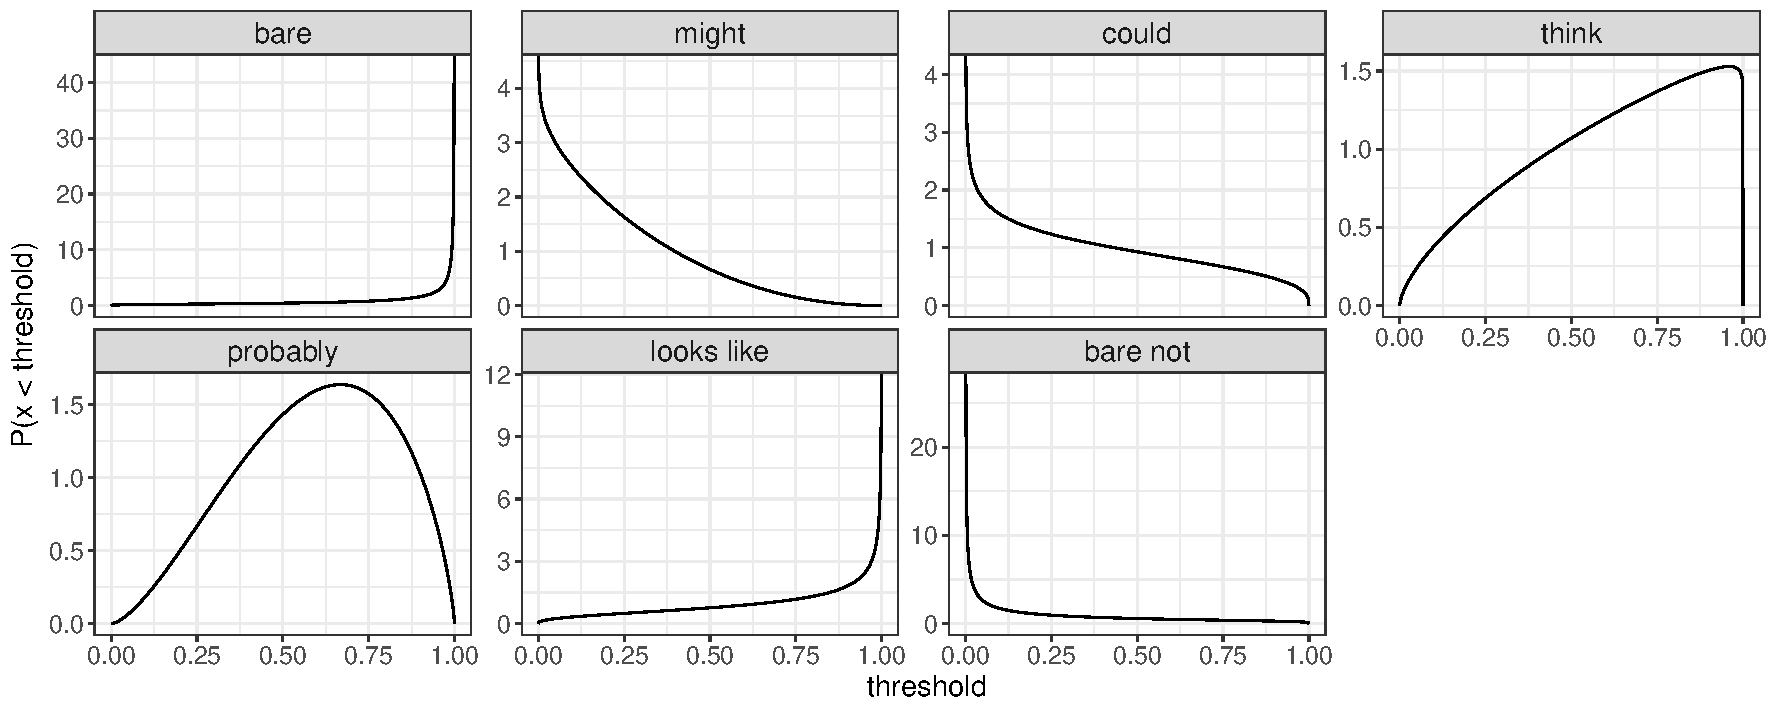
\includegraphics[width=\textwidth]{plots/threshold-distributions-prior.pdf}
\caption{Inferred threshold distributions. \label{fig:threshold-distributions}}
\end{figure}

Overall, despite some small deviations between the model predictions and participants' behavior, our model
seems to be a plausible model of participants' average expectations of utterance choices in different
situations. And as we will see in Section~5, this model is also well suited to capture participants' prior beliefs
about an unknown speaker's utterance choices.



\section{Experiment 1: Adaptation of Speaker Expectations}

We now turn to our main research questions of whether and how listeners adapt to variable uses of uncertainty expressions.
In our norming studies, we found that participants show variation and uncertainty in their expectations about a generic speaker's 
use of \textit{might} and \textit{probably}. Based on these results, we investigate in this experiment whether participants update 
their expectations about the use of uncertainty expressions of a specific speaker after observing this speaker's use of 
uncertainty expressions for a short period of time. The procedure, materials and analyses were pre-registered at \url{https://osf.io/w926x/}.


\subsection{Participants}
We recruited a total of 80 participants (40 per condition) on Amazon Mechanical Turk. 
We required participants to have a US-based IP address and a minimal approval rating 
of 95\%. Participants were paid \$2 which amounted to an hourly wage of approximately 
\$12--\$15. None of the participants had previously participated in the norming study.

\subsection{Materials and Procedure}

\paragraph{Exposure trials:} In the first part of the experiment, participants saw 20 exposure trials. 
These trials had a similar setup as the trials in the norming study: 
they also showed a child requesting a blue or orange gumball and a gumball machine with blue and orange gumballs. 
However, instead of the cartoon adult, they showed a video of an adult male or female speaker (counterbalanced across participants) producing one of the following six utterances:

\begin{itemize}
\item You'll get a blue/orange one (\textsc{bare})
\item You might get a blue/orange one (\textsc{might})
\item You'll probably get a blue/orange one (\textsc{probably})
\end{itemize}

\begin{table}
\centering
\begin{tabular}{l c c c c c c}
\toprule
& \multicolumn{2}{c}{\sc might} & \multicolumn{2}{c}{\sc probably} & \multicolumn{2}{c}{\sc bare}\\
& $n$ & $\phi$ & $n$ & $\phi$ & $n$ & $\phi$\\
\midrule
\emph{cautious} & {\bf 10} & {\bf 60\%} & 5 & 90\% & 5 & 100\%\\
\emph{confident} & 5 & 25\% & {\bf 10}  & {\bf 60\%} & 5  & 100\%\\  
\bottomrule
\end{tabular}
\caption{Number of exposure trials ($n$) per utterance ({\sc might}, {\sc probably}, {\sc bare}) and associated proportion of target color gumballs ($\phi$) in the \emph{cautious} vs.~\emph{confident} speaker conditions. Critical trials bolded. \label{tab:materials}}

\end{table}

The number of trials with each of these utterances as well as the gumball proportions varied across two conditions (see Table \ref{tbl:materials} for an overview). In the {\it confident speaker} condition, participants saw 10 critical trials with 60\% target color gumballs and the speaker producing an utterance with \emph{probably} (target color was randomized across trials), 5 filler trials with 100\% target color gumballs and the speaker producing {\sc bare}, and 5 filler trials with 25\% target color gumballs and the speaker producing {\sc might}. In the {\it cautious speaker} condition, participants saw 10 critical trials with 60\% target color gumballs and the speaker producing an utterance with \emph{might}, 5 filler trials with 100\% target color gumballs and the speaker producing {\sc bare}, and 5 filler trials with 90\% target color gumballs and the speaker producing {\sc probably}. The filler trials were intended to boost confidence in the speaker and contained event probability-utterance combinations, which were rated highly in the norming study. 

Participants were instructed to watch what the speaker had to say to the child. The video started automatically after a 400ms delay and participants had the option to replay the video as often as they wanted. To advance to the next scene, participants had to press a button which was disabled until the video clip had finished.

\paragraph{Test trials:} The test phase was almost identical to the  \textit{might-probably} condition of the norming study except that the cartoon figure of the man was replaced with a picture of the speaker that participants saw on the exposure trials. Participants were presented with scenes containing gumball machines with 9 different proportions of blue and orange gumballs  (identical as in the norming study) and they were asked to provide ratings for the utterances {\sc might} and {\sc probably} by distributing 100 points across these two utterances and the blanket {\it something else} option. Participants provided two ratings for each of the 18 color-gumball machine combinations resulting in a total of 36 trials. 

Both speakers were from the East Coast and Native Speakers of North American English.\footnote{The first author compensated each of the speakers for their help with the recordings with two slices of marble Guglhupf.} They were instructed to produce the utterances in a normal voice without any special prosody.


\paragraph{Attention checks}  In order to verify that participants were paying attention to the video and the scenes, we included 15 attention checks (6 during exposure and 9 during test trials), which were randomly positioned within the two experimental phases. Trials that contained an attention check either displayed or did not display (pseudo-randomized) a small grey X somewhere around the gumball machine. After completing a trial with an attention check, participants were asked whether they had seen a grey X in the previous scenes or not.

\subsection{Exclusions} We excluded participants who provided incorrect responses to more than 3 of the catch trials. Based on this criterion, we excluded 11 participants in the \textit{confident speaker} condition and 8 participants in the \textit{cautious speaker} condition. None of the results reported below depend on these exclusions.


\subsection{Analysis and Predictions}  

Intuitively, a more confident speaker uses {\sc probably} for a larger and {\sc might} for a smaller range of event probabilities than a more cautious speaker. 
Therefore, if participants track these different uses, we expect their ratings to depend on how the speaker used uncertainty expressions during the exposure phase. 
Following \cite{Yildirim2016}, we quantified this prediction by fitting a spline with four knots for each expression and each participant and computing the area 
under the curve (AUC) for the splines corresponding to each expression and participant. The area under the curve is proportional to how highly and for how large 
of event probabilities participants rate an utterance. If an utterance is rated highly for a larger range of event probabilities, the AUC will also be higher. 
We therefore tested whether listeners updated their expectations according to these intuitions by computing the difference between the AUC of the spline for 
{\sc might} and of the spline for {\sc probably} for each participant. We predicted that the mean AUC difference would be higher in the 
\emph{cautious speaker} condition than in the \emph{confident speaker} condition.

\subsection{Results and Discussion}

\begin{figure}
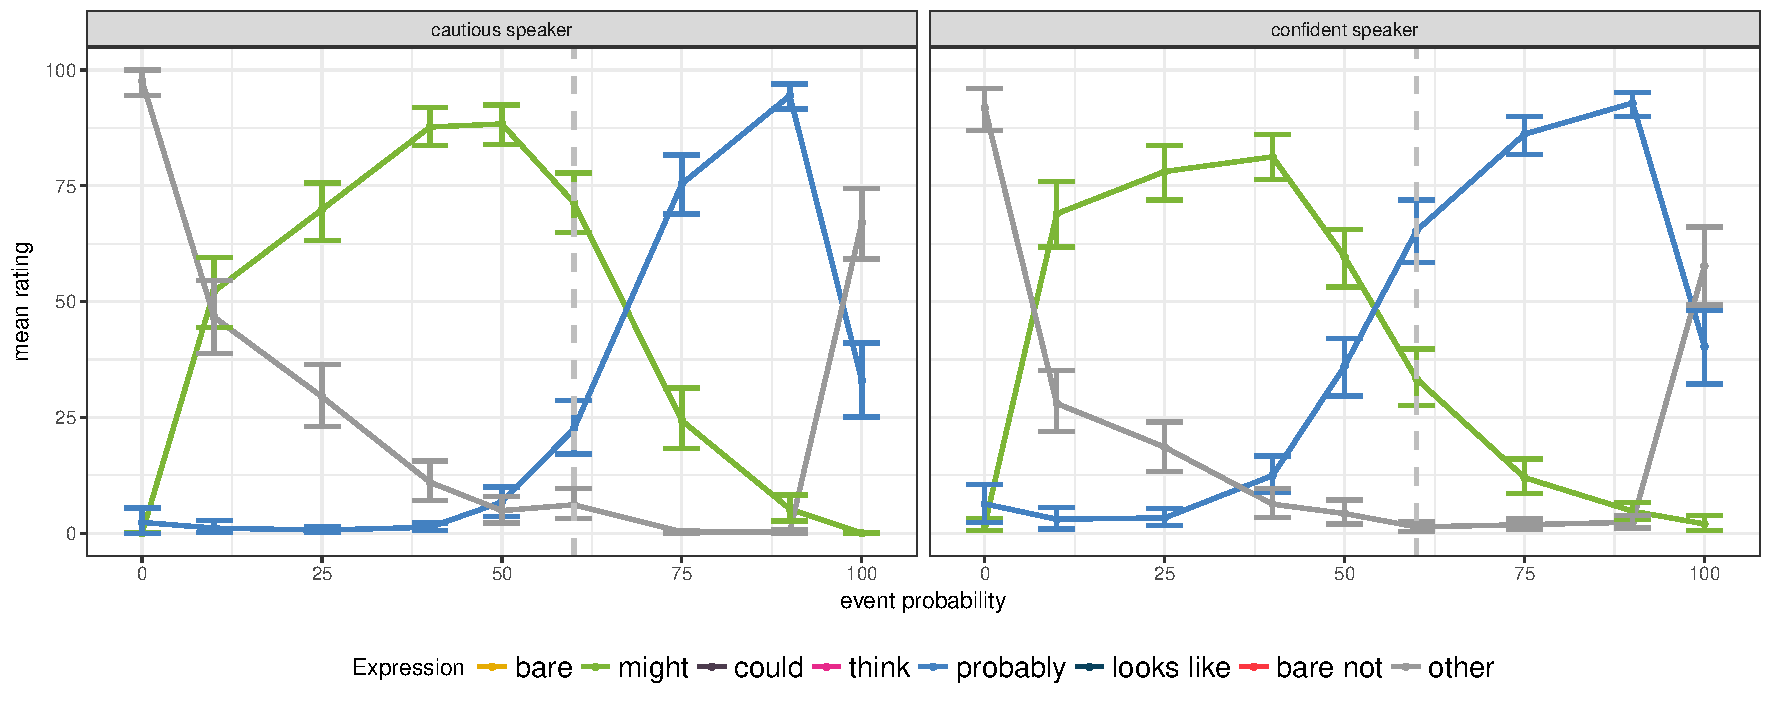
\includegraphics[width=\textwidth]{plots/exp-1-ratings.pdf}
\caption{Mean post-exposure ratings from Experiment 1. Error bars correspond to bootstrapped 95\%-confidence intervals.  The grey dotted line highlights the ratings for the 60\% event probability ratings.  \label{fig:adaptation-results-prod}}
\end{figure}

\begin{figure}
\center
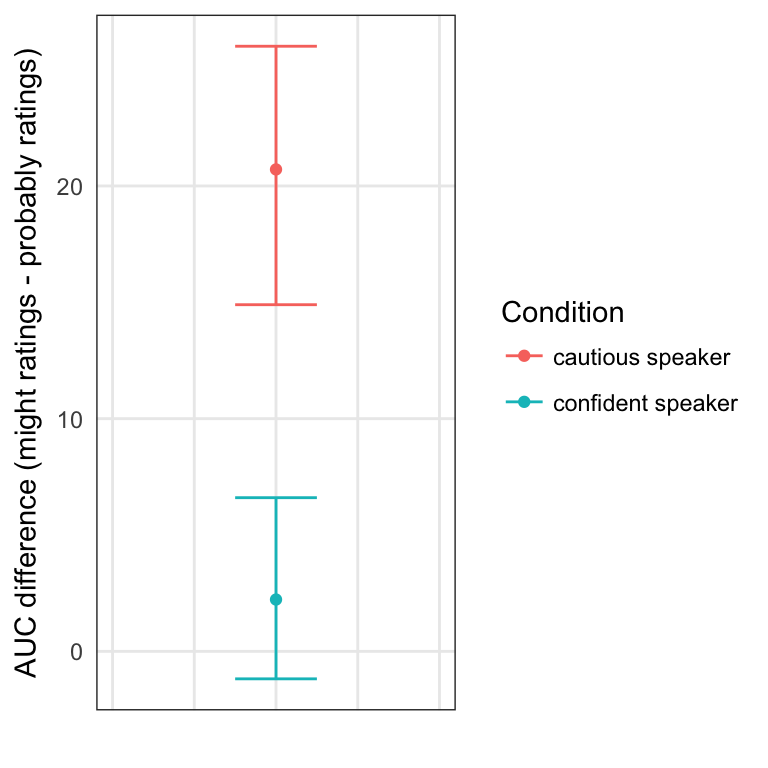
\includegraphics[width=.5\textwidth]{plots/adaptation-auc-production.png}
\caption{Area under the curve (AUC) differences from Experiment 1. Error bars correspond to bootstrapped 95\%-confidence intervals.  \label{fig:adaptation-auc-prod}}
\end{figure}

Figure~\ref{fig:adaptation-results-prod} shows the mean ratings for the three options in the two conditions. As these plots show, participants updated their expectations about the speaker's language use and therefore made different predictions about how the speaker would use uncertainty expressions. In the \emph{cautious speaker} condition, participants gave high ratings for {\sc might} for a larger range of event probabilities than in the \emph{confident speaker} condition. On the other hand, participants gave high ratings for {\sc probably} for a larger range of gumball proportions in the \emph{confident speaker} condition than in the \emph{cautious speaker} condition. These differences result in a significantly greater AUC difference in the \emph{cautious speaker} condition than in the \emph{confident speaker} condition ($t(59) = 4.98$, $p < 0.001$, see also Figure~\ref{fig:adaptation-auc-prod}).

As Figure~\ref{fig:adaptation-results-prod} shows, participants also differed in their ratings of the two utterances when they were presented with a scene with 60\% target color gumballs. In the {\emph cautious speaker} condition, participants rated {\sc might} higher than {\sc probably}; in the {\emph confident speaker} condition, the pattern was reversed and participants rated {\sc probably} higher than {\sc might}. These expectations mirror the speaker behavior during the exposure phase and provide additional evidence that participants tracked the speaker's usage of uncertainty expressions. 

Our results also seem to rule out several alternative explanations. If we  considered only the ratings for {\sc might} and {\sc probably}, an alternative explanation for the results would be that participants did not form speaker-specific expectations about the mapping between event probabilities and uncertainty expressions but were instead inferring different higher-level goals of the speakers. For example, it could be that participants in the \emph{confident speaker} condition were inferring from the speaker's language use that the speaker wanted to be very encouraging towards the child. While this seems prima facie a reasonable explanation, we would then also expect participants' ratings of \emph{ something else} for high event probabilities to differ across the two conditions. If participants inferred that the adult wants to be highly encouraging, then we would expect that participants assumed that the adult used more encouraging language when there is a high probability of getting a target color gumball. This in return should lead participants to give higher ratings to the \emph{something else} option for high event probabilities, which we did not observe in this experiment. In fact, numerically, the rating of \emph{something else} was higher in the \emph{cautious speaker} condition than in the \textit{confident speaker} condition.

Further, we can also rule out that participants were only learning something about the speaker's preferences for different uncertainty expressions. One potential objection to our experiment is that the number of utterances with {\sc might} and {\sc probably} differed across the two conditions (see Table~\ref{tbl:materials}) and a possible alternative explanation for our results is that participants learned that the {\it cautious speaker} overall prefers to use {\sc might} and the {\it connfident speaker} prefers {\sc probably}. To rule out this possibility, we conducted a replication of our experiment with equal number of exposures to both utterances in both conditions. In this replication, we again found a greater AUC difference in the \emph{cautious speaker} condition than in the \emph{confident speaker} condition ($t(58) = 3.12$, $p < 0.01$).

In summary, taking all these results together, our experiment provides evidence for listener adaptation to a specific speaker's use of uncertainty expressions after a brief exposure phase.

% 

\section{Adaptation model}

The experimental results presented in the previous section suggest that listeners are updating some expectations about language use when they are interacting with a speaker. 
However, what kind of expectations listeners are updating is unclear. It could be that listeners are updating their expectations about the speaker's lexicon 
(i.e., the mapping between event probabilities and uncertainty expressions); it could be that listeners are updating their expectations about the speaker's preferences; and
it could be that listeners are updating their expectations about both the speaker's lexicon and the speaker's preferences.

We investigate what kind of expectations listeners are updating through a series of simulations of the adaptation process. Crucially, we assume that in interaction,
listeners form beliefs about a set of speaker-specific parameters $\Theta_S$. 
We further assume that the formation of these beliefs is an instance of Bayesian belief updating:
listeners start off with prior beliefs about $\Theta_S$ based on their general knowledge about 
language and subsequently update their beliefs about $\Theta_S$ with every production. 
That is, after observing a series of productions $D={d_1, ..., d_n}$ where each $d_i$ is an 
utterance-event probability pair $d_i = (u_i, \phi_i)$, listeners beliefs about $\Theta_S$ are the result
of performing Bayesian inference:
$$P(\Theta_S \mid D) \propto P(\Theta_S) P(D \mid \Theta_S) = P(\Theta_S) \prod_{i=1}^nP(d_i \mid \Theta_S) $$

\noindent We assume that the likelihood function is the \textit{expected speaker} $ES_1$ parameterized by $\Theta_S$:

$$P(\Theta_S \mid D) \propto P(\Theta_S)  \prod_{i=1}^n ES_1(u_i \mid \phi_i, \Theta_S) $$



\subsection{Simulations}

Our adaptation model crucially relies on a prior over speaker-specific parameters $P(\Theta_S)$
which reflects listeners prior beliefs about the use of uncertainty expressions. For our simulations,
we assume that the estimates of the model parameters that we obtained from fitting the model
to the norming data corresponds to the means of this prior distribution.

In order to investigate which kind of parameters are updated during adaptation, we run simulations
with different priors:

\begin{itemize}
\item \textbf{\textit{Cost}}: We use a normal distribution centered at the mean value that we inferred from the norming data for the prior over cost parameters. Unlike in the norming study, we now assume that each expressions has its own cost parameter reflecting the expressions's preferences. We use a delta distribution, i.e., a distribution with zero variance, for the priors over all other parameters.
\item \textbf{\textit{ Threshold distributions}}:  We parameterize the Beta distributions $P(\theta_u)$ with their mean $\mu_u$ and population parameter $\nu_u$ \citep{Kruschke2014}. We use a truncated normal distribution $\mathscr{N}_{[0,1]}$ centered at the mean value from the norming data for the means of the Beta distributions $\mu_u$. We use a delta distribution for the priors over all other parameters, including the population parameters $\nu_u$.\footnote{The population parameters govern the variance of a Beta distribution such that higher population parameters result in lower variance of the distribution. It is quite likely that the population parameter also changes during adaptation but to keep the number of moving parts in our model to a minimum, we decided to keep these parameters constant.}
\item \textbf{\textit{ Cost and threshold distributions}}: We use a normal distribution for the prior over cost parameters and a truncated normal for the prior over the means of the threshold distributions. We use a delta distribution for the priors over all other parameters.
\end{itemize}

Each of these priors corresponds to a different hypothesis in terms of what kind of expectations listeners are updating during adaptation: the {\it cost} prior corresponds to the hypothesis that listeners are updating their beliefs about speaker preferences; the {\it threshold distributions} prior corresponds to listeners updating beliefs about the underlying threshold distributions; and the {\it cost and threshold distributions} prior corresponds to listeners updating beliefs about preferences and threshold distributions. To adjudicate between these three hypotheses, we ran simulations of the adaptation process for both conditions with different priors and compared the models in terms of their likelihood of generating the experimental data.

For each condition, we used the same priors and then performed Bayesian inference to infer the posterior distribution after observing the 20 utterances that participants had seen in the exposure phase (see Table~\ref{tbl:materials} for an overview of the 20 utterances in the two conditions). We performed inference using MCMC with a Metropolis-Hastings sampler. We used thinning of 10, discarded the first 2,000 burn-in samples and collected 10,000 samples per chain. We ran two chains and confirmed that the chains had converged using the $\hat{R}$ criterion. 

We used the following standard deviation values for the prior distributions.
\begin{itemize}
\item \textbf{Cost}: $\sigma_{cost} = 0.1$ (for the two expressions that participants can choose from, i.e., \textit{might} and \textit{probably}) and $\sigma_{cost} = 0.5$ for all other expressions.
\item \textbf{Threshold distribution mean}: $\sigma_{\mu_u} = 0.05$.
\end{itemize}

\noindent We believe that these values are reasonable but they were not estimated from data or otherwise derived in a formal manner. We
did not optimize these values in order to limit the experimenter degrees of freedom.


\subsection{Model comparisons}

We compare the models in terms of two factors. First, we consider the correlation between participants' average post-exposure ratings and the maximum a posteriori predictions of the post-exposure model. Second, we compute the likelihood of the model generating the post-exposure data. For the latter, we constructed a dataset $D_{obs}$ of utterance-event probability pairs by treating each post-exposure rating as a probability distribution and sampling 10 utterances from it. We then computed the posterior likelihood odds between Model 1 with posterior distribution over parameters $P(\Theta_{S}^{(1)})$ and Model 2 with posterior distribution $P(\Theta_{S}^{(2)})$.

$$\mbox{posterior likelihood odds} = \frac{\mathlarger{\int_0^1} {P\left(\Theta_{S}^{(1)}\right) P\left(D_{obs} \mid \Theta_{S}^{(1)} \right) d   \Theta_{S}^{(1)}}}{\mathlarger{\int_0^1} P\left(\Theta_{S}^{(2)}\right) P\left(D_{obs} \mid \Theta_{S}^{(2)}\right)d   \Theta_{S}^{(2)} }$$
 
\noindent The posterior likelihood odds indicate how much more likely it is that the data was generated by Model 1 than by Model 2. Since we are marginalizing out a distribution over parameter values, this comparison of models will naturally
favor simpler models. For a more complex model with more parameters, the distribution over different parameter values will be more disperse and can contain more parameter configurations that lead to a low likelihood of the data.

\begin{table}
\center
\begin{tabular}{r | c | c | c | c }
\multicolumn{1}{c }{} & \multicolumn{2}{c  }{cautious speaker} & \multicolumn{2}{c  }{confident speaker}  \\
Model & $R^2$ &   odds &  $R^2$ &    odds  \\ \midrule
prior & 0.791 & 10^{-526} & 0.703 & 10^{-437} \\
cost & 0.906 & $ 10^{-302}$ & 0.796 & $ 10^{-147}$  \\
threshold distributions & 0.834 & $10^{-118}$ & 0.915& $10^{-57}$ \\
cost \& threshold distributions & 0.948 & 1 & 0.837 & 1\\
\end{tabular}
\caption{Model evaluation results. $R$\textsuperscript{$2$} are the correlations between the mean post-exposure ratings and the model predictions. \textit{odds} are the posterior likelihood odds of the models compared to the \textit{cost and threshold distributions} model. \label{tbl:model-comparison}}
\end{table}

\begin{table}
\center
\begin{tabular}{r | c | c | c | c }
\multicolumn{1}{c }{} & \multicolumn{2}{c  }{cautious speaker} & \multicolumn{2}{c  }{confident speaker}  \\
Model & $R^2$ &   odds &  $R^2$ &    odds  \\ \midrule
prior & 0.736 & 10^{-529} & 0.596 & 10^{-491} \\
cost & 0.868 & $ 10^{-416}$ & 0.806 & $ 10^{-163}$  \\
threshold distributions & 0.816 & $ 10^{-237}$ & 0.928& $10^{-23}$ \\
cost \& threshold distributions & 0.922 & 1 & 0.883 & 1\\
\end{tabular}
\caption{Model evaluation results on replication of Experiment~1. $R$\textsuperscript{$2$} are the correlations between the mean post-exposure ratings and the model predictions. \textit{odds} are the posterior likelihood odds of the models compared to the \textit{cost and threshold distributions} model. \label{tbl:model-comparison-replication}}
\end{table}

Table~\ref{tbl:model-comparison} shows the correlations of the three models with the experimental data as well as the
 posterior likelihood odds. As the values in this table show, the model in which the cost as well as the threshold 
 distributions are updated during adaptation is much more likely to generate the experimental data than the other 
 two less complex models. This is also reflected in the correlations between the model predictions and the average 
 ratings, which are the highest (or approximately equally high) for the model which allows both types of parameters 
 to be updated as compared to the other two models. This all suggests that listeners are indeed updating their beliefs 
 about preferences as well as the threshold distributions when adapting to a speaker's use of uncertainty expressions.

We further replicated these results by running another set of simulations to predict the post-adaptation ratings for both 
conditions from the replication of Experiment~1 (now exposing the model to 5 additional utterances). The model 
evaluation results for these simulations are shown in Table~\ref{tbl:model-comparison-replication}. As the values
in this table show, the models in which both the costs and the threshold distributions can be updated is again more
likely to generate the experimental data than the other two models.

In summary, all our modeling experiments strongly suggest that listeners are updating their beliefs about speaker
preferences as well as speaker's threshold distributions.

\subsection{Model evaluation}

\begin{figure}
  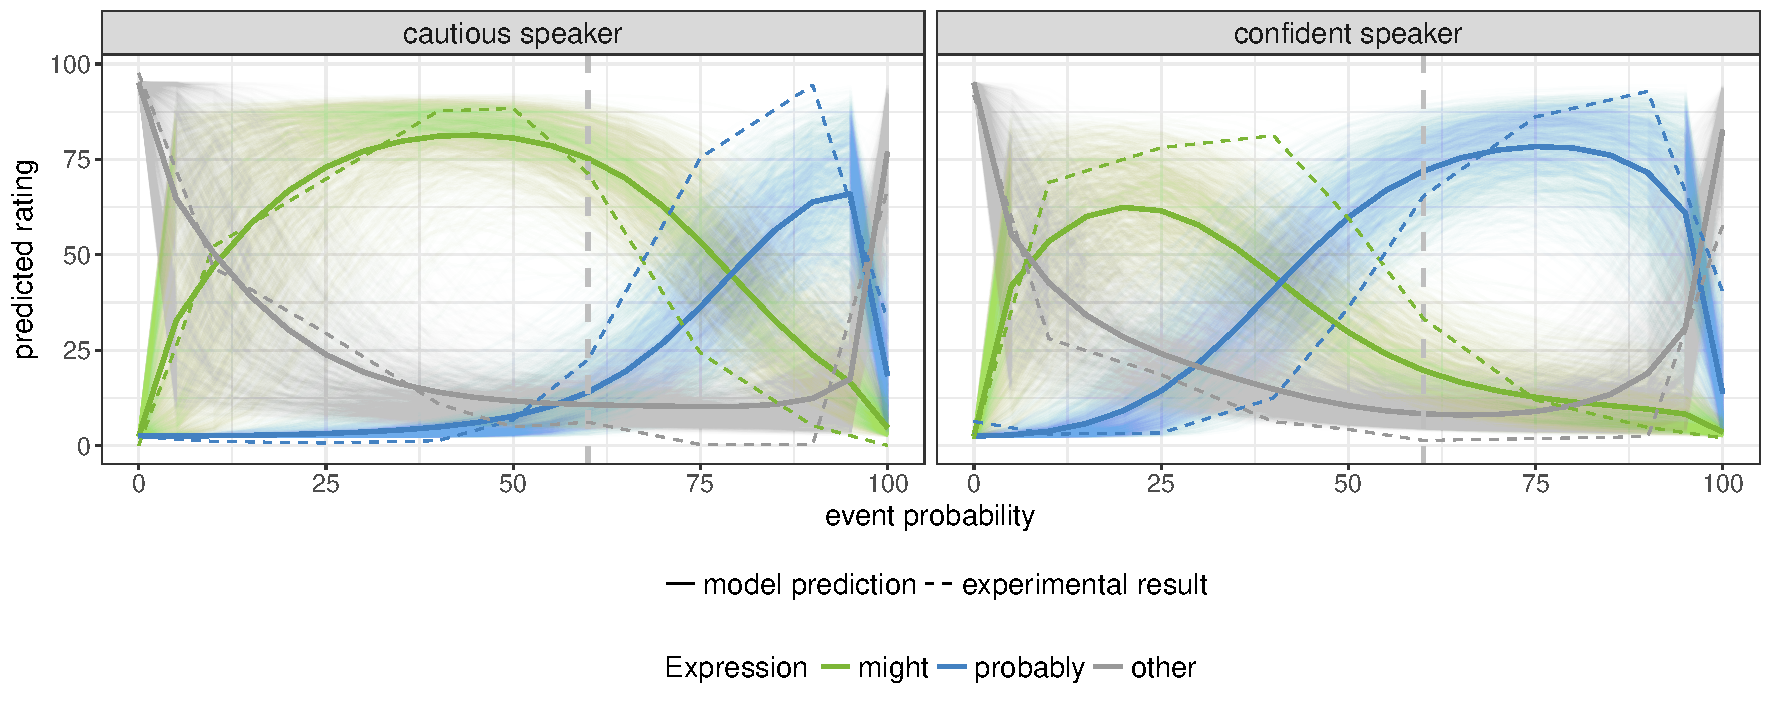
\includegraphics[width=\textwidth]{plots/adaptation-posterior-predictions.pdf}
  \caption{Post-adaptation model predictions and experimental results. 
  The solid lines shows the mean model predictions and the shades around the mean indicate the distribution of the model predictions. \label{fig:post-exposure-model}}
\end{figure}

Figure~\ref{fig:post-exposure-model} shows the post-exposure predictions as well as the average participant ratings for the two conditions. As these plots show, the model
predictions are similar to participants' ratings but also show clear deviations. This is not surprising considering that we did not fit the model to the experimental data  but
rather obtained the predictions by simulating the adaptation process. The most prominent deviation is that  participants' ratings are more extreme than the model predictions. 
At the same time, however, the model also makes several correct predictions. Most crucially, it predicts that in the \textit{cautious speaker} condition, ratings for {\sc might} are higher than {\sc probably} when
the event probability is 0.6 and that in the \textit{confident speaker} condition, {\sc probably}  is rated higher than {\sc might}. Further, it also correctly predicts for very low
event probabilities, a higher rating for \textsc{might} in the \textit{confident speaker} condition than in the \textit{cautious} speaker condition.

We can also again inspect the inferred model parameters. Figures~\ref{fig:post-exposure-thresholds} and \ref{fig:post-exposure-costs} compare the inferred
post-exposure threshold distributions and costs between the two conditions and the prior. As expected, the means of the threshold distributions for \textit{might} and \textit{probably} 
decreased when simulating adaptation to the \textit{confident speaker} whereas they slightly increased when the model adapted to the \textit{cautious speaker} condition.
The threshold distributions for the other expressions did not shift. This is also expected since the uses of {\sc bare} in the exposure phase was compatible with the priors and
none of the other utterances were used during the exposure phase. For the inferred cost parameters, we observe the following changes. The costs for all utterances that are not mentioned
during exposure do not differ from the prior. This was the same for the  { \sc might} and {\sc probably} utterances. The cost for the \textsc{bare} utterance, on the other hand, decreased.
This is again expected since the prior over the costs for {\sc might} and {\sc probably} is centered at a much lower value because of 
our condition-specific cost function in the norming study. The prior over the cost for {\sc bare}, on the other hand, is centered at a higher value but since the model was
exposed to multiple {\sc bare} utterances in the simulations, it learned that the speaker has higher preference for {\sc bare}.

\begin{figure}
  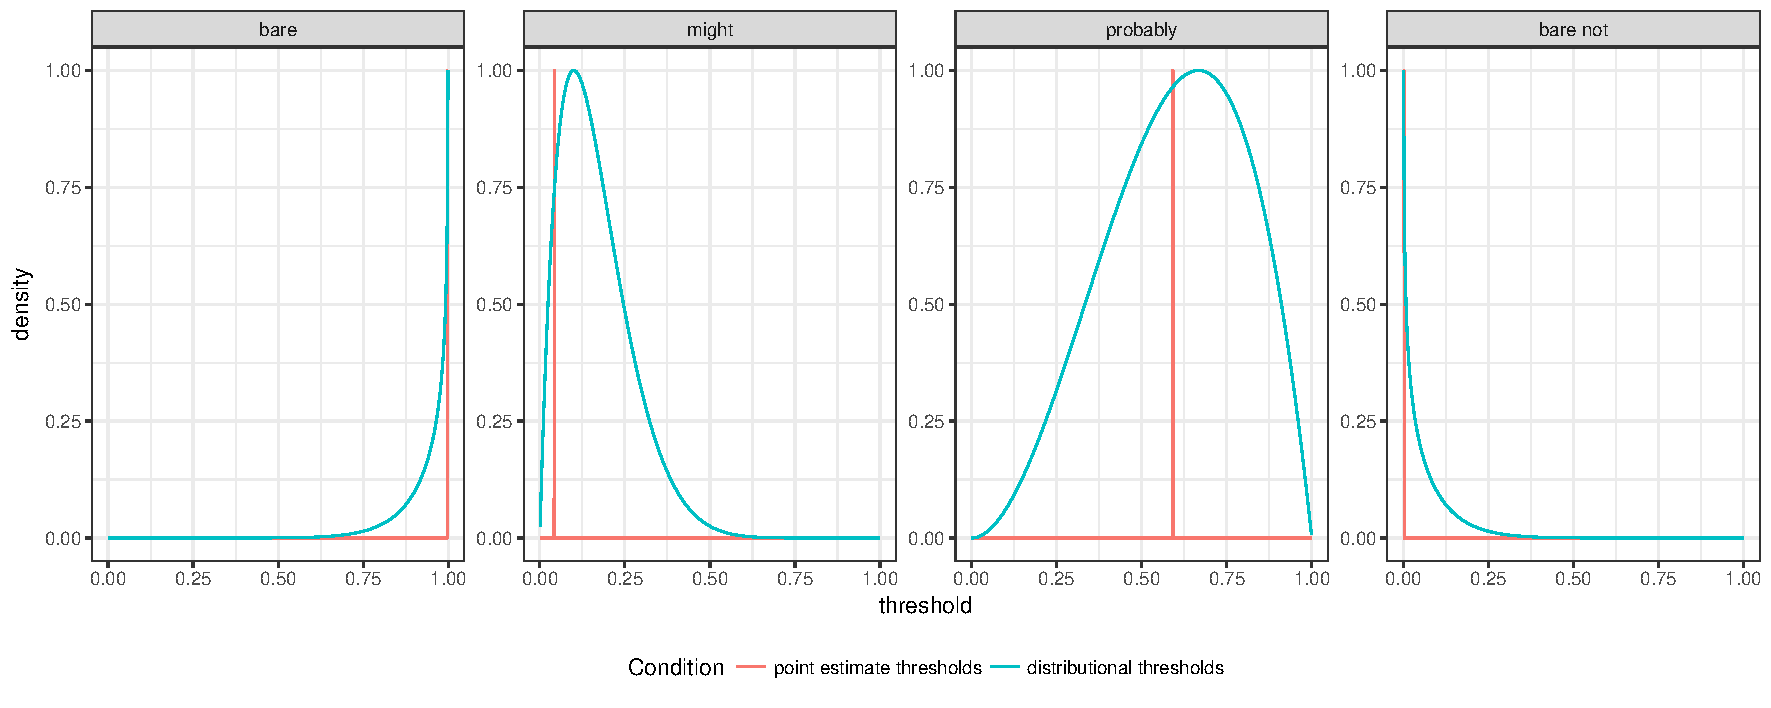
\includegraphics[width=\textwidth]{plots/adaptation-posterior-thresholds.pdf}
  \caption{Post-adaptation threshold distributions. \label{fig:post-exposure-thresholds}}
\end{figure}

\begin{figure}
\center
  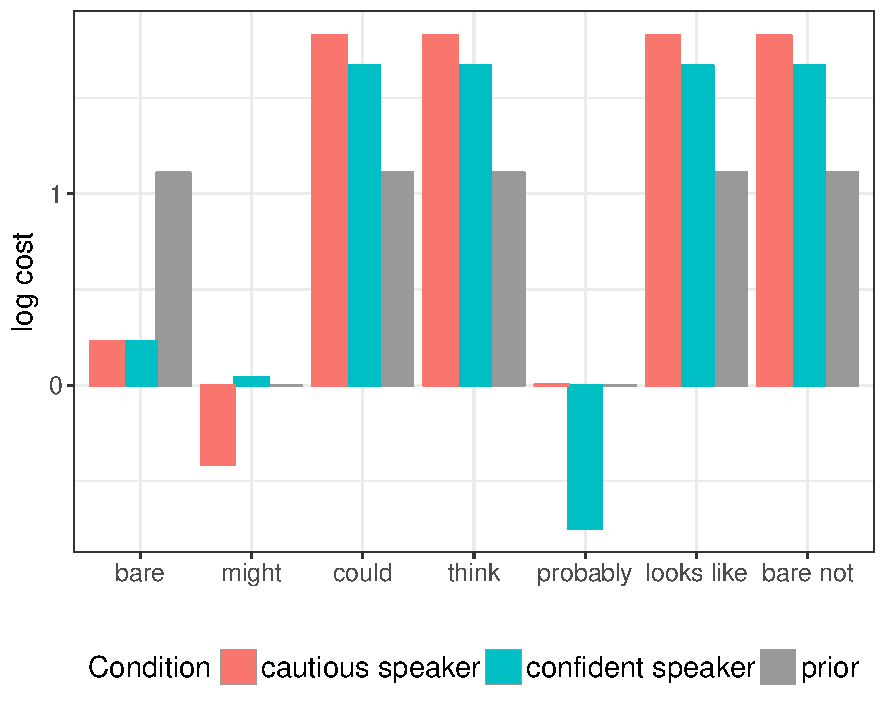
\includegraphics[width=0.5\textwidth]{plots/adaptation-posterior-costs.pdf}
  \caption{Post-adaptation cost values. \label{fig:post-exposure-costs}}
\end{figure}




\section{Adaptation of interpretations}

\begin{figure}
  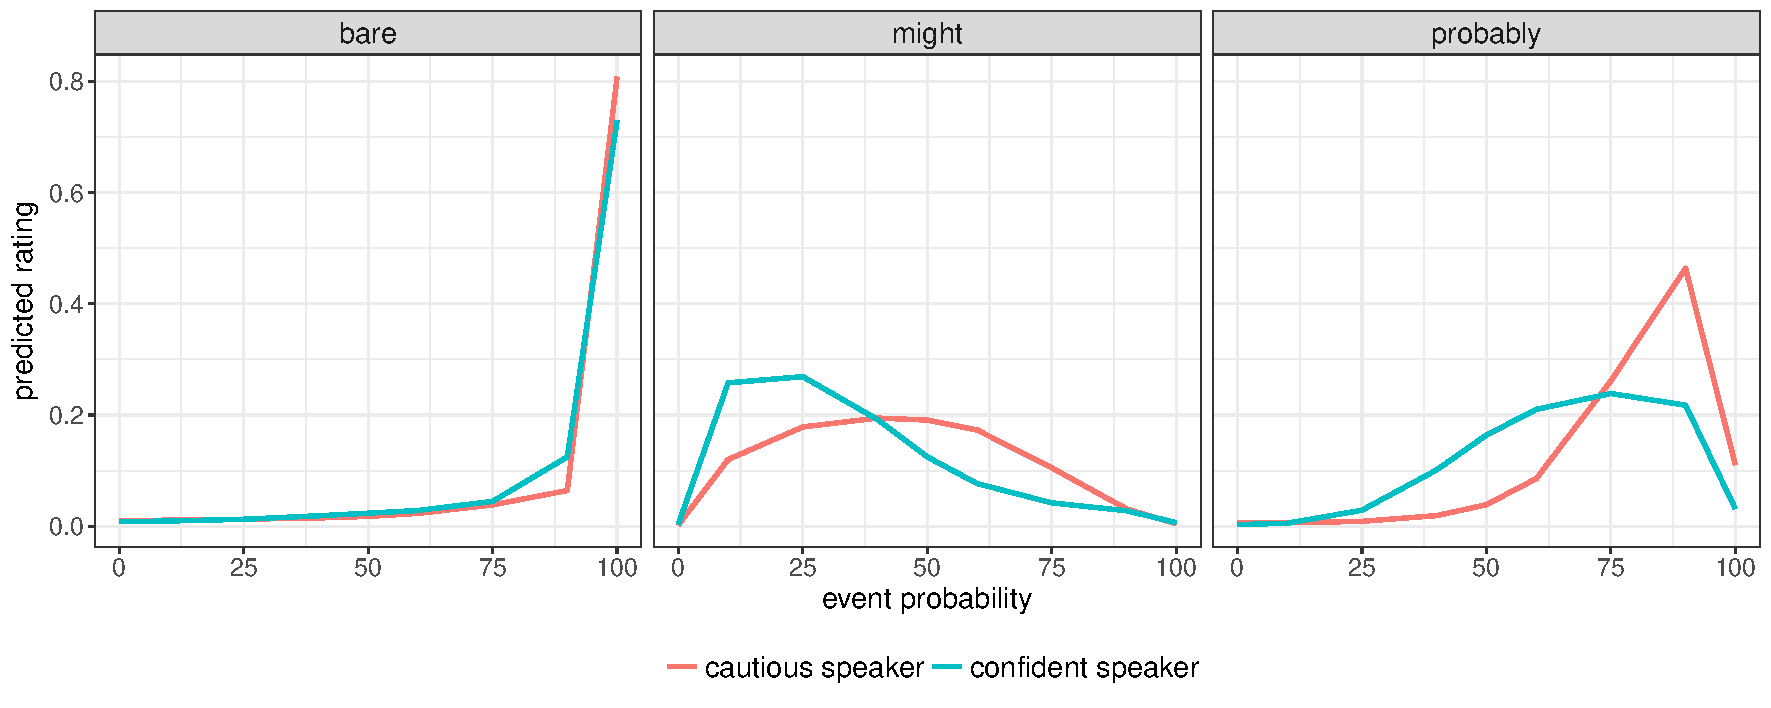
\includegraphics[width=\textwidth]{plots/adaptation-posterior-comp.pdf}
  \caption{Post-adaptation interpretation distribution. \label{fig:post-exposure-comp}}
\end{figure}


Up to this point, we have made the implicit assumption that listeners' expectations about a speaker's language use guide their interpretations. This behavior is
predicted by RSA models, which assume that a pragmatic listener $L_1$ tries to infer the state of the world (in our case, the event probability $\phi$) by reasoning
about their prior beliefs about the world state and their expectations about a speaker's language use (in our case, the expected pragmatic speaker $ES_{1}$).

$$ L_1(\phi \mid u) \propto P(\phi) ES_1(u \mid \phi)$$

According to such a model of interpretation, the shifts in expectations that we observed in the previous experiment, should also lead to a shift in interpretations. 
If we again assume a uniform prior over event probabilities, then our model predicts that listeners who were exposed to a \textit{cautious} speaker should infer 
higher event probabilities when hearing {\sc might} or {\sc probably} than listeners who were exposed to a \textit{confident} speaker. Figure~\ref{fig:post-exposure-comp}
shows the distribution over event probabilities after hearing three different utterances as predicted by $L_1$ parameterized by the inferred parameters from our
adaptation simulations in the previous section. As these plots show, in the \textit{cautious speaker} condition, the distribution over event probabilities after hearing \textit{might} 
and \textit{probably} is shifted towards higher values as compared to the distributions in the \textit{confident speaker} condition. 

In our second experiment, we tested whether this prediction is correct and whether listeners' change in expectations transfers to a change in interpretations. 
The procedure, materials and analyses were pre-registered at \url{http://bitly.com/2SpMPaZ}.

\subsection{Participants}

We recruited a total of 80 participants (40 per condition) on Amazon Mechanical Turk. We required participants to have a US-based IP address and a minimal approval rating of 95\%. Participants were paid \$2 which amounted to an hourly wage of approximately \$10--\$12. None of the participants had participated in any of the previous experiments. 

\subsection{Materials and Procedure}

Participants completed a set of exposure trials followed by a set of test trials. The exposure trials were identical to the exposure trials in Experiment~1. The test trials probed participants' interpretations of the utterances {\sc might}, {\sc probably} and {\sc bare}. In each test trial, participants listened to a recording of the speaker from the exposure phase producing {\sc might}, {\sc probably} and {\sc bare} and then participants were asked to rate for 9 gumball machines with the same proportions of blue and orange gumballs as in the previous experiments how likely they thought it was that the speaker saw each of these gumball machines by adjusting a slider. All 9 gumball machines were presented at the same time but to avoid visual clutter, all gumball machines except the one whose slider participants were adjusting had an opacity of 0.1 and the animation was disabled. Participants provided 9 ratings per trial and completed in total 6 trials -- one for each expression-color pair. The exposure phase contained again 6 attention check as in the previous experiment. However, given the low attention check performance in the previous experiment, we modified one aspect about the attention checks: We always displayed the grey X on the first trial with an attention check so that participants would see the gray X before being presented with the attention check. We discarded answers to the first attention check and computed the attention check performance on the remaining 5 attention checks.

\subsection{Exclusions}

We excluded participants who failed more than 2 attention checks, which led to 2 exclusions in the \emph{cautious speaker} condition and 1 exclusion in the \emph{confident speaker} condition.


\subsection{Analysis and Predictions}

If participants reason about the speaker and update their expectations of a specific speaker, we also expect that participants interpretations 
vary depending on which speaker they were exposed to. Concretely, we expect that listeners interpret a more confident speaker's utterance 
to communicate a lower event probability than a more cautious speaker's utterance. We tested this prediction by treating participant's ratings 
of gumball machines as a probability distribution over gumball proportions (and consequently event probabilities).  For each utterance, we 
normalized participants ratings of the different gumball machines so that they summed up to 1, so that we could interpret the normalized scores 
as a categorical probability distribution over gumball machines given an utterance. We computed the expected value of blue gumballs from these probability distributions and compared these expected values across the two conditions. We predicted that the expected values of {\sc might} and {\sc probably} were going to be larger in the \emph{cautious speaker} condition than in the \emph{confident speaker} condition.

\subsubsection{Results and Discussion}

\begin{figure}
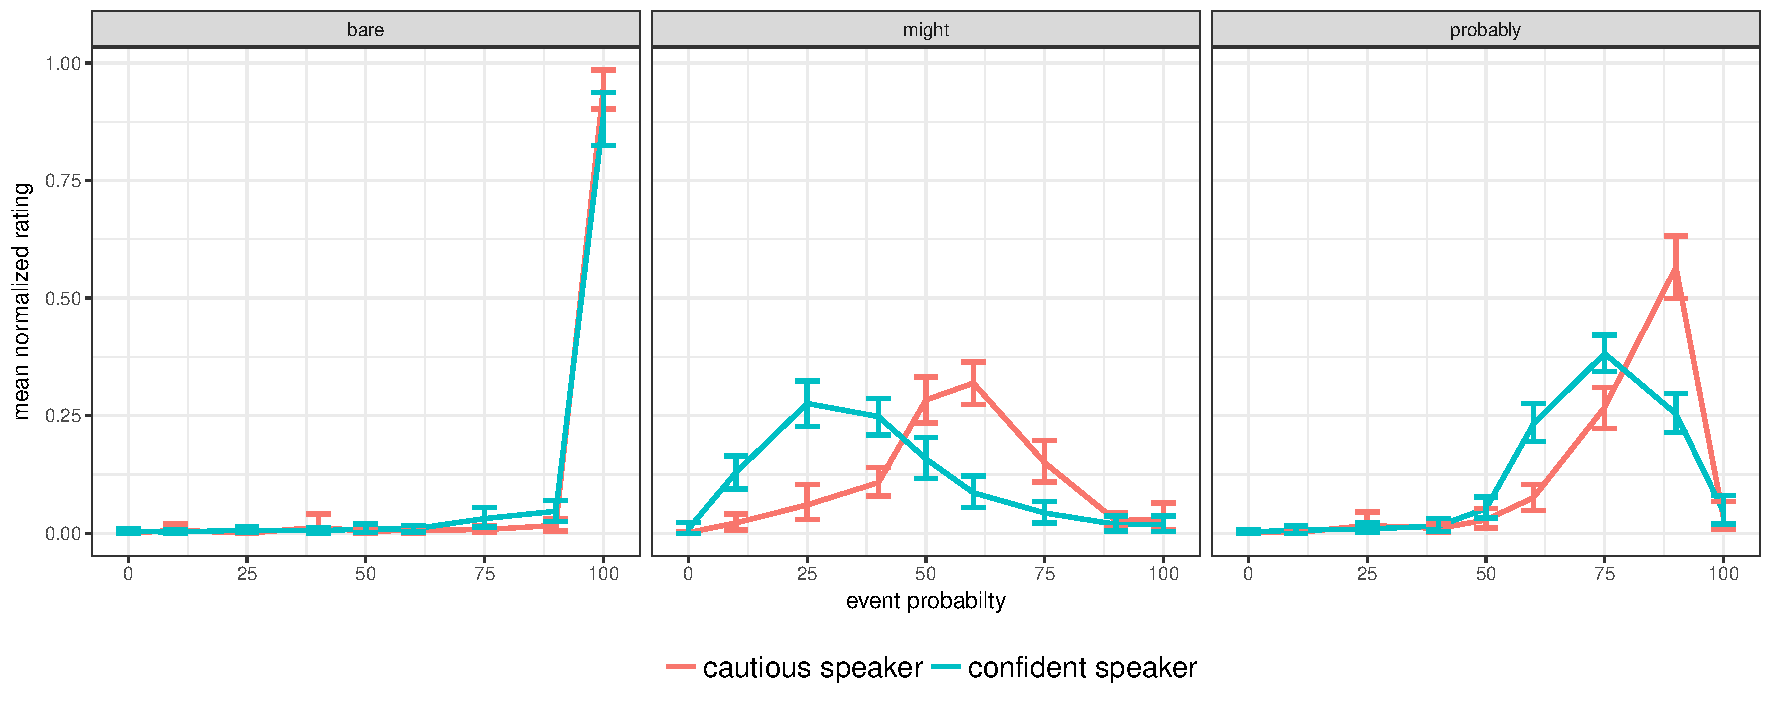
\includegraphics[width=\textwidth]{plots/exp-2-ratings.pdf}
\caption{Aggregated post-exposure ratings from Experiment~2.  \label{fig:adaptation-results-comp}}
\end{figure}

\begin{figure}
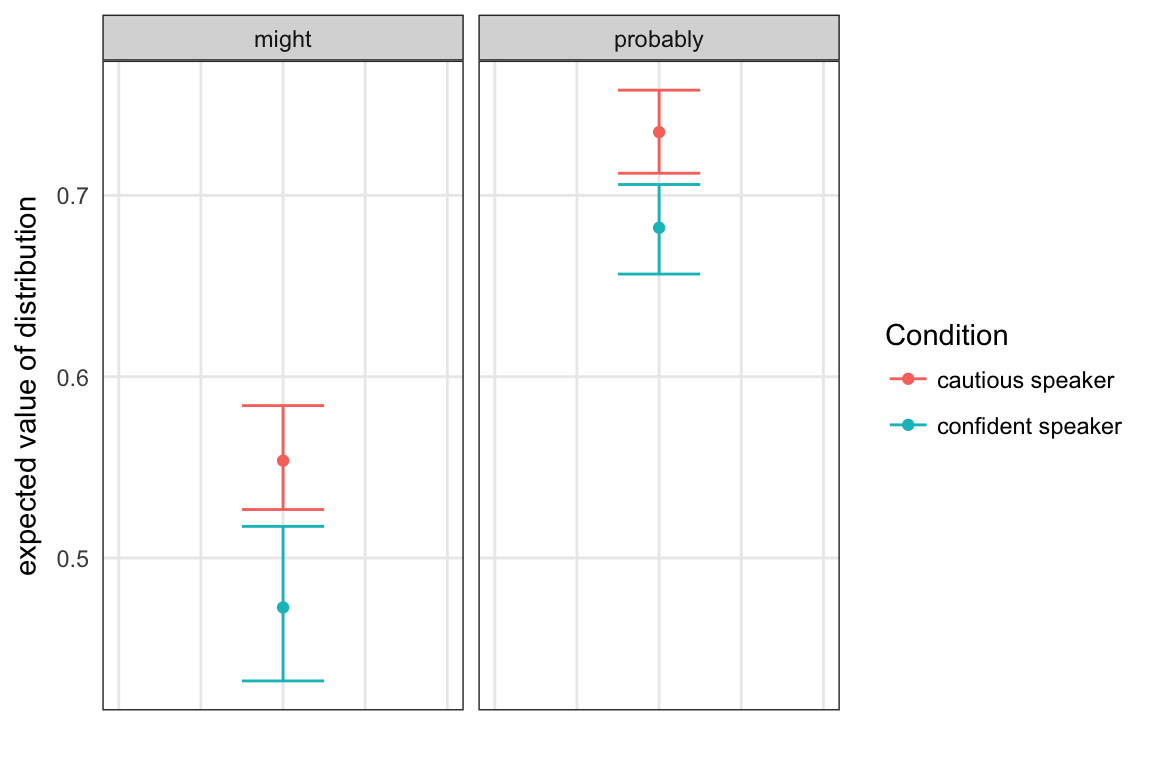
\includegraphics[width=.75\textwidth]{plots/adaptation-diff-comprehension.png}
\caption{Expected values for {\sc probably} and {\sc might} from Experiment~2.  \label{fig:adaptation-exp-comp}}
\end{figure}


Figure~\ref{fig:adaptation-results-comp} shows the aggregated and normalized ratings for the two conditions.  As predicted, participants provided higher ratings for gumballs with higher target color percentages after hearing {\sc might} and {\sc probably} in the \emph{cautious speaker} condition than in the \emph{cautious speaker} condition. This also led to a significantly higher expected value for {\sc might} ($t(75)=3.05$, $p<0.01$) and {\sc probably} ($t(75)=3.08$, $p<0.01$, see also Figure~\ref{fig:adaptation-exp-comp}) in the \emph{cautious speaker} condition as compared to the \emph{confident speaker} condition.

These results suggest that listeners not only update their expectations of what a speaker is likely to say in different situations but that also their interpretations of uncertainty expressions adapt to specific speakers.


\section{General Discussion}

{\bf TODO} 

* talk about findings

provides evidence that bayesian belief updating is also a suitable model for higher-level linguistic tasks
priors are important




* contributions
	
	* marrying RSA with speaker-specific beliefs
	
	 * paradigm for studying uncertainty expressions
	
	 * latent semantics approach

 	 * dealing with uncertainty doesn't only seem to be true for lower-level processing but also higher-level processing
	 
	  * fits right into all the literature about language processing
	
	other things:
	
	*  memory mechanisms unclear but seems compatible with Horton \& gerrig and other memory processes
	
	* question about associative memory vs. error correction (still unclear) (look again at Brown-schmidt)
	
 	*  our approach similar to hawkins2017 and bergen, levy \& goodman
	
	*  relationship to pogue et al.
	
	*  discuss the unnatural nature of our experiment --$>$ not interactive (common in reading, news, ....); observed both world state
	     and the utterance --$>$ admittedly slightly unnatural but could be that one reads the weather report later or that people keep track
	     over time how likely events following what a person said
	     
       * wittenberg


future directions:

* talk about adaptation to multiple speakers

* talk about testing other predictions about the model

* long-term speaker-specific mappings
	

\printbibliography
%\bibliography{qp-references}


%=====================================================================

%\begin{addresses}
 % \begin{address}
%    Author1 \\
%    Street \\
%    \ldots \\
%    \email{author1@email}
%  \end{address}
%  \begin{address}
 %   Author2 \\
 %   Street \\
 %   \ldots \\
 %   \email{author2@email}
 % \end{address}
 % ...
%\end{addresses}

%=====================================================================


\section*{Supplementary material}

\subsection*{Effect of color in norming study}

As mentioned in a footnote, we ran the norming studies in three batches using three slightly different procedures across conditions. We originally ran condition 0 (\emph{bare-might}) as a pilot condition. In the results, we noted that participants did not differ in their ratings depending on whether the girl asked for a blue or an orange gumball ($R^2(27)=0.997$ between mean ratings for blue and orange trials). To lower the number of trials, we therefore asked each participant to provide ratings for only one of the two colors (randomized across participants) for the next batch of conditions (conditions 1-14). We found that in some conditions, this led to small differences in ratings between participants who always rated utterances with \emph{blue} and participants who always rated utterances with \textit{orange} ($R^2(27)$ between $0.864$ and $0.984$). We hypothesize that this is a result of participants paying less attention if they were asked to do exactly the same task over and over again (in condition 0, the color potentially changed across trials). In order to verify the stability of our results, we replicated one of the conditions, condition 5 (\emph{might-probably}), and had participants provide two ratings for each color and gumball proportion. We found that despite the lower correlation between average ratings for utterances with \emph{blue} and utterances with \emph{orange} in the original run ($R^2(27)=0.929$), there was a very high correlation between the average ratings independent of the color of the original study and the average ratings of the replication ($R^2(27)=0.975$), which suggests that the average ratings largely do not depend on whether we ask participants to provide ratings for both colors or just one color. Nevertheless, we used the modified procedure in which we asked participants to provide 2 ratings for each color and gumball proportion for the last batch of conditions (conditions 15-20). In all conditions in which we asked people to provide ratings for utterances with both colors, the correlation between average ratings for utterances with \emph{blue} and utterances with \emph{orange} was almost perfect ($R^2(27)>0.988$).

\subsection*{Additional pre-exposure ratings}

\begin{figure}
\includegraphics[width=\textwidth]{plots/pre\string_test\string_s1.pdf}
\caption{Results of norming study -- Part 1. Error bars correspond to bootstrapped 95\%-confidence intervals. \label{fig:norming-results-1}}
\end{figure}

\begin{figure}
\includegraphics[width=\textwidth]{plots/pre\string_test\string_s2.pdf}
\caption{Results of norming study -- Part 2. Error bars correspond to bootstrapped 95\%-confidence intervals. \label{fig:norming-results-2}}

\end{figure}

\begin{figure}
\includegraphics[width=\textwidth]{plots/pre\string_test\string_model\string_s1.pdf}
\caption{Model predictions and results from norming study -- Part 1. Error bars correspond to 95\% high density intervals (model predictions) and bootstrapped 95\%-confidence intervals (observed results). \label{fig:norming-results-model-1}}

\end{figure}

\begin{figure}
\includegraphics[width=\textwidth]{plots/pre\string_test\string_model\string_s2.pdf}
\caption{Model predictions and results from norming study -- Part 2. Error bars correspond to 95\% high density intervals (model predictions) and bootstrapped 95\%-confidence intervals (observed results). \label{fig:norming-results-model-2}}

\end{figure}

%\section{Models}
%
%While the results of the two experiments suggest that there is considerable variation in the use of uncertainty expressions and that listeners can adapt their speaker expectations after listening to a speaker several times, the experimental results do not explain the adaptation process. We therefore also attempt to model participant behavior using a Bayesian cognitive model. In particular, we are investigating whether adaptation is a result of participants learning the speaker's  utterance {\bf preferences}, learning the speaker's {\bf meanings} of uncertainty expressions (i.e., which range of probabilities does an uncertainty expression map to in this specific context) or a combination of learning speaker {\bf preferences} and {\bf meanings}.
%
%\subsection{Overview}
%
%We model adaptation as Bayesian belief updates about the {\bf meanings} of uncertainty expressions and utterance {\bf preferences}. Formally, let $\Theta_S$ be the set of parameters that governs the meaning of uncertainty expressions used by speaker $S$ as well as the utterance preferences by $S$. We assume that a listener updates their beliefs about $\Theta_S$ after hearing a specific speaker produce utterances with uncertainty expressions along with observations that allow the listener to infer the probability of an event happening, i.e., after experiencing set $\mathscr{D}$ of $(u, \phi)$ observations, a listener updates their beliefs about $\Theta_S$\footnote{Similar models have also been proposed by \cite{Qing2013} and \cite{Hawkins2017} for adaptation to different uses of quantifiers and convention formation, respectively.}:
%
%$$P(\Theta_S \mid \mathscr{D}) \propto P(\Theta_S) P(\mathscr{D} \mid \Theta_S) = P(\Theta_S) {\textstyle \prod_{(u, \phi) \in \mathscr{D}} } S_1(u \mid \phi; \Theta_S).$$
%
%\noindent Here, we assume that the likelihood of the set of observations $\mathscr{D}$ is the likelihood of producing utterances $u$ given an event probability $\phi$ according to a speaker model $S_1$ parametrized by $\Theta_S$. We now discuss both this speaker model $S_1$ as well as the prior distribution $P(\Theta_S)$ in turn.
%
%\subsection{Speaker-specific production and comprehension model}
%
%We model production and comprehension within the Rational Speech Act (RSA) framework \citep{XXX}. We follow previous work on uncertainty expressions \citep{Lassiter2013,Herbstritt2017} and assume that uncertainty expressions have a threshold semantics, i.e., an utterance with an uncertainty expression  $u$  is semantically felicitous if it denotes a proposition that has probability $\phi$, which exceeds a threshold $\theta_u$:
%
%$$L_0(\phi \mid u, \theta_u) \propto P(\phi) \times \mathbbm{1}\left[\phi > \theta_u\right]$$ 
%
%A pragmatic speaker $S_1$ (our production model) then chooses her utterance to communicate that an event will happen with probability $\phi$ by soft-maximizing her speaker utility 
%$$EU_S(\phi, u) =  \int_0^1 {P_S\left(\theta_U\right) \log L_0(\phi \mid u, \theta_u) d\theta - c_S(u) },$$ which is the difference of the negative surprisal of the listener and the speaker-specific utterance cost $c_S(u)$.  Here, we also assume that in choosing an utterance, a speaker samples a threshold $\theta_u$ from probability distributions $P_S\left(\theta_u\right)$ which represent $S_1$'s beliefs about reasonable thresholds.
%
%
%$$S_1(u \mid \phi) \propto   \exp \lambda U_S\left(\phi, u \right),$$
%
%\noindent where $P_S(\theta) = \prod_{u \in U}P_S(\theta_u)$ and $\lambda$ is a rationality parameter which governs the optimality of the speaker choice. A pragmatic listener $L_1$ (our comprehension model)  interprets these utterances by reasoning about the speaker:
%
%$$L_1(\phi \mid u) \propto P(\phi) S_1(u \mid \phi).$$
%
%\noindent Our speaker-specific model crucially depends on two speaker-specific functions, namely the distributions over thresholds $P_S(\theta_u)$ and the cost function $c_S(u)$. We assume that each $P_S(\theta_u)$ follows a Beta distribution with parameters $\alpha_{Su}$ and $\beta_{Su}$. Beta distributions seem well-suited for two reasons: First, $\theta_u$ always has to be within the interval $[0,1]$, which is identical to the support of a Beta distribution, and second, Beta distributions can take many different shapes and we expect that for some uncertainty expressions, most of the probability mass is concentrated at one of the endpoints. For the cost function, we assume that a speaker's utterance cost is a constant depending on the uncertainty expression $c_S(u)=\gamma_{Su}$. The utterances that we are considering are all of approximately equal length, so we assume that the cost term primarily captures speaker preferences rather than processing costs. 
%
%\subsection{Priors}
%
%Adult listeners are experts in language use in their native language and hence we expect them to have very strong prior expectations on how speakers use language. We encode this prior knowledge in the prior $P(\Theta_S)$. We assume that this prior is the joint probability of all parameters in $\Theta_u$, which we assume to be independent. Beta distributions can be parametrized in numerous ways (see e.g., \cite{Kruschke2014}) which can make inference easier or harder  and avoid potentially degenerate solutions. For adaptation, we reparameterize the Beta distributions over thresholds $\theta_{Su}$ using the distribution mean $\mu= \frac{\alpha}{\alpha + \beta}$ and the population size parameter $\nu=\alpha + \beta$. We assume that the prior parameters follow the following distributions:
%
%$$\mu_u \sim \mbox{TruncatedNorm}(\mu_{\mu_u}, \sigma_{\mu_u}, 0, 1) \qquad \nu_u \sim \mbox{Log-Norm}(\mu_{\nu_u}, \sigma_{\nu_u}) $$
%$$ \gamma_u \sim \mbox{Log-Norm}(\mu_{\gamma_u}, \sigma_{\gamma_u})$$
%
%$\mu_u$ always has to be within the interval $[0,1]$ and within that it seems to roughly follow a Normal distribution, therefore we opted for a truncated normal as a prior for these parameters. $\nu_u$ and $\gamma_u$ on the other hand, always have to be greater than 0 and a log-normal distribution seems to describe the distribution of parameters very well.
%
%\subsubsection{Mean estimation}
%
%We estimated the parameters for the prior as well as the rationality parameter $\lambda$ from the norming study using Bayesian data analysis. We treated each participants rating over utterances in a trial as a probability distribution over utterances given an event probability $\phi$ and we sampled 10 utterances from each of these distributions, resulting in a set $\mathscr{E}$ of utterance/probability pairs $(u, \phi)$. We then estimated the means of the prior distributions over parameters $\theta_S$, i.e., $\mu_{\mu_u}$, $\mu_{\nu_u} $  and $\mu_{\gamma_u}$ for each utterance $u$ by estimating the MAP values of the posterior distribution 
%
%$$P(\theta_S, \lambda \mid \mathscr{E}) = P(\theta_S, \lambda) P(\mathscr{E} \mid \theta_S, \lambda) = P(\theta_S, \lambda) \prod_{(u,\phi) \in \mathscr{E}} S_1'(u \mid \phi, \theta_S, \lambda).$$ 
%
%$S_1'$ is a modified version of the speaker-specific production model $S_1$ which makes a few additional assumptions with respect to the data collection.
%
%\begin{enumerate}
%\item Instead of $c(u)$, we use a special condition-specific cost function:
%$$
%c(u, condition) = 
%     \begin{cases}
%       0 &\quad\text{if } u  \text{ is one of the utterances in } condition\\
%       \gamma &\quad\text{otherwise} \\
%     \end{cases}
%$$
%\item We include a noise term and we assume that in 5\% of the cases participants chose a random utterance.
%\item We assume the set of possible utterances is comprised of the seven utterances with uncertainty expressions that we mentioned above, i.e., $U = \{$ {\sc bare}, {\sc might}, {\sc probably}, {\sc could}, {\sc think}, {\sc looks like}, {\sc bare not}$\}$
%\item We assume that $$S_1'(\mbox{\textit{``other''}} \mid \phi, \mbox{condition}) \propto O + \sum_{u \in U \land u \not \in \mbox{condition}} S_1(u \mid \phi)$$
%\item Speaker-specific parameters $\Theta_S$ are shared across all participants.
%\end{enumerate}
%
%The rationale behind assumption (i) is that we only provide participants with two utterance choices and the blanket \emph{other} response in the norming study and therefore we expect that participants will be heavily primed to use the two provided utterances whenever they are semantically felicitous, which we can model with our condition-specific cost function. Also note that we assume that all utterances have the same cost  $\gamma$ if they are not part of the current condition. We made this choice based on the finding that the model tended to overfit the data when we allowed each of these parameters to vary independently, and as mentioned earlier, given that all the utterances have approximately the same length, we don't expect that participants have strong expectations about the preferences of a speaker a priori to encountering the actual speaker. 
%
%The rationale behind assumption (ii) is that as in any web-based experiment, we will have participants who make random choices, do not pay attention, or make mistakes, and we do not want that noise to influence our actual parameter estimation. This is in particular important for expressions that tend to have very high thresholds $\theta_u$. For example, a rational participant who pays attention is highly unlikely to assign a rating above 0 to the utterance ``You'll get a blue one'' if the objective probability of getting a blue gumball is 0\% and we want this to be reflected in our distribution $P\left(\theta_{\mbox{bare}}\right)$. However, if a few participants who either did not pay attention or made mistakes provide non-zero ratings for this utterance/probability combination, this could skew the threshold distribution considerably towards 0, which is something we want to avoid.
%
%The reason for assumption (iii) is that we only collected data for this set of utterances and that the RSA model the way we specified here requires a fixed set of utterances.
%
%Finally, in our experiments, participants cannot freely choose among all utterances that they would be able to produce in a more naturalistic setting. We therefore assume that they reason about other utterances which include the 5 utterances that were not part of the respective condition as well as other utterances that we are not even considering here. This is captured by the fact that we are summing over all the other utterances and an inferred constant $O$, which is intended to capture the probability of all utterances that we didn't consider in any of the conditions.
%
%
%
%\subsubsection{Variance estimation}
%
%\subsubsection{Implementation details}
%
%We implemented the model in Python using {\tt numpy} and {\tt scikit-learn} libraries. We used MCMC with the  Metropolis-Hastings algorithm. For the MAP estimation, we collected 100,000 MCMC samples after discarding the first 20,000 burn-in samples. This samples were obtained by collecting  a sample at every 10th iteration (i.e., we used thinning of 10). For the bootstrapping procedure, we collected 20,000 MCMC samples of each run and discarded the first 10,000 burn-in samples. Again, we thinned the chain by collecting samples at every 10th iteration. 
%
%We used the following proposal distributions for the various parameters:
%
%$$\alpha_u^{(t)} \sim \mbox{Log-Norm}(\alpha_u^{(t-1)}, XXX) $$
%$$\beta_u^{(t)} \sim \mbox{Log-Norm}(\beta_u^{(t-1)}, XXX)  $$
%$$\gamma^{(t)} \sim \mbox{Log-Norm}(\gamma^{(t-1)}, XXX)$$
%$$\lambda^{(t)} \sim \mbox{Uniform}(\lambda^{(t-1)}-XXX, (\lambda^{(t-1)}+XXX)$$
%
%
%Uninformed priors. 
%
%\subsubsection{Inferred parameters}
%
%\subsubsection{Model predictions and criticism}
%
%
%
%\subsection{Pre-test experiment}
%
%\subsubsection{Model}
%
%We model the process that leads to the experimental results in the pre-test experiment as a speaker model ($S_1$) in the Rational Speech Acts framework \citep{RSA}. We assume that participants take the role of a generic speaker but given that they reason about a non-specific speaker, participants have some uncertainty about the speaker's language use.
%
%Within the RSA framework, a pragmatic speaker reasons about a literal listener ($L_0$). In the context of our experiment, we define the following literal listener in a similar vain as Lassiter and Goodman (2015) and Herbstritt and Franke (2017). 
%$$L_0(\phi \mid u; \theta) \propto P(\phi) \left( {0.95} \times \mathbbm{1}[\phi > \theta_{u}] + 0.05 * P_{uniform}(\phi; 0,1) \right)$$
%
%The literal listener tries to infer the probability $\phi$ of an event happening (in our case, the probability of getting a blue gumball) from an utterance with an uncertainty expression $u$. We assume that for each uncertainty expression, there is some threshold $\theta_u$ such that $u$ is semantically felicitous if  $\phi$ is above this threshold. We assume that the prior $P(\phi)$ is uniform. Given that we are dealing with noisy experimental data, we also include a noise term of the form $0.05 * P_{uniform}(\phi; 0,1)$, which allows for random inferences in 5\% of the cases. 
%
%\vspace{1em}
%
%\textbf{Q:} Is this a reasonable way to model noise?
%
%\vspace{1em}
%
%
%We assume that each uncertainty expression has its own threshold, except for the negated version of the bare statement, which we assume to be true if $\phi$ is less than $1-\theta_{bare}$ (Herbstritt and Franke, 2017).
%
%Given this literal listener, a pragmatic speaker $S_1$, tries to maximize the listener's utility when choosing an utterance to communicate the probability $\phi$. We assume that a speaker chooses among the 6 utterances that were used across the 15 conditions and the the negated version of the bare statement, i.e., \textit{"You won't get a blue one"}.
%$$S_1( u \mid \phi, condition; \theta ) \propto exp \left(\lambda \left( \log P_L(\phi \mid u; \theta) - c(u, condition) \right) \right) $$
%
%Following the vanilla RSA model, we define the utility as the negative surprisal subtracted by the cost of the utterance. Given our experimental setting in which we ask participants to choose between two given utterances and \textit{other}, we use the following cost function, which depends on the experimental condition.
%$$
%c(u, condition) = 
%     \begin{cases}
%       0 &\quad\text{if } u  \text{ is one of the utterances in } condition\\
%       c_{u} &\quad\text{otherwise} \\
%     \end{cases}
%$$
%
%The motivation here is that participants will be primed to use the two given utterances, which is reflected in the lower cost.
%
%The $S_1$ model that we presented here is still parameterized by a set of thresholds $\theta$. Considering the variation in use of uncertainty expressions, participants seem to show uncertainty about how a generic speaker would set $\theta$ for the individual uncertainty expressions. We therefore assume that participants come with a prior over reasonable thresholds and given that they are asked to reason about an unknown speaker, they marginalize over this prior to derive the distribution over utterances, which results in the following revised speaker model.
%
%$$P_S(u \mid \phi, condition) \propto \int P(\theta) exp\left(\lambda  \left(\log P_L(\phi \mid u; \theta) - c(u, condition)\right)\right) d\theta $$
%
%\subsubsection{Parameter estimation}
%
%Our model has 14 parameters, namely 6 prior distributions over thresholds $P(\theta_u)$, 7 cost terms $c_u$, and the rationality parameter $\alpha$, which we all estimate from the experimental data. For the prior distributions $P(\theta_u)$, we assume that these follow a beta distribution parametrized by $\alpha_u$ and $\beta_u$ (Qing (2014) made similar assumptions for modeling the use of \textit{some} and \textit{many}). There are two main reasons for choosing a beta distribution: First, its range is from 0 to 1, and given that $\theta$ defines a threshold parameter for a probability, this matches exactly the reasonable interval for the thresholds. Second, the beta distribution can take very different shapes and therefore we are not making the assumption that all of the prior distributions over thresholds have a similar shape.
%
%To facilitate computations, we discretize our speaker and listener model as well as the priors over thresholds and infer these distributions by enumerating all possibilities. To estimate the model parameters, we run MCMC with 8,000 burn-in samples and 12,000 samples.\footnote{Note that this does not seem to be enough samples yet as 3 different runs still lead to varying results and don't pass the criterion by Gelman and Rubin (1992). I'm currently running the model again with 100,000 samples, which will hopefully be enough for stable parameter estimates.} 
%
%We sample parameters from the following distributions.
%
%$$\alpha_u, \beta_u \sim Uniform(0,30)$$
%$$c_u\sim Uniform(0,5)$$
%$$\lambda \sim Uniform(0.1,3)$$
%
%We then estimate the parameters by computing the distributions over parameters given the experimental data across all 15 conditions $\mathscr{D}$.
%
%\begin{align*}
%P(\alpha,\beta, c, \lambda \mid \mathscr{D}) &\propto P(\alpha, \beta, c, \lambda) P(\mathscr{D} \mid \alpha,\beta, c, \lambda) \\
%&= P(\alpha, \beta, c, \lambda) \prod_{d \in \mathscr{D}} P_S(u_d \mid \phi_d, condition_d; \alpha, \beta, c, \lambda)
%\end{align*}
%
%Note that for each probability $\phi$, participants provided a distribution over utterances and not actual samples of utterances given $\phi$. For each trial in which a participant provided a distribution over utterances, we therefore sampled 10 utterances from this distribution and combined all of these samples to form the data $\mathscr{D}$ from which we estimated the parameters of our model.
%
%For each parameter, we take the median of the 12,000 MCMC samples and use these parameter estimates for making model predictions.
%
%
%\subsubsection{Model predictions}
%
%The following plots show the experimental results (left) and the model predictions (middle) for several (representative) conditions.\footnote{See \url{https://github.com/sebschu/adaptation/blob/master/models/1_threshold_modals/prediction_model.html} for results for all 15 conditions.}
%
%\begin{center}
%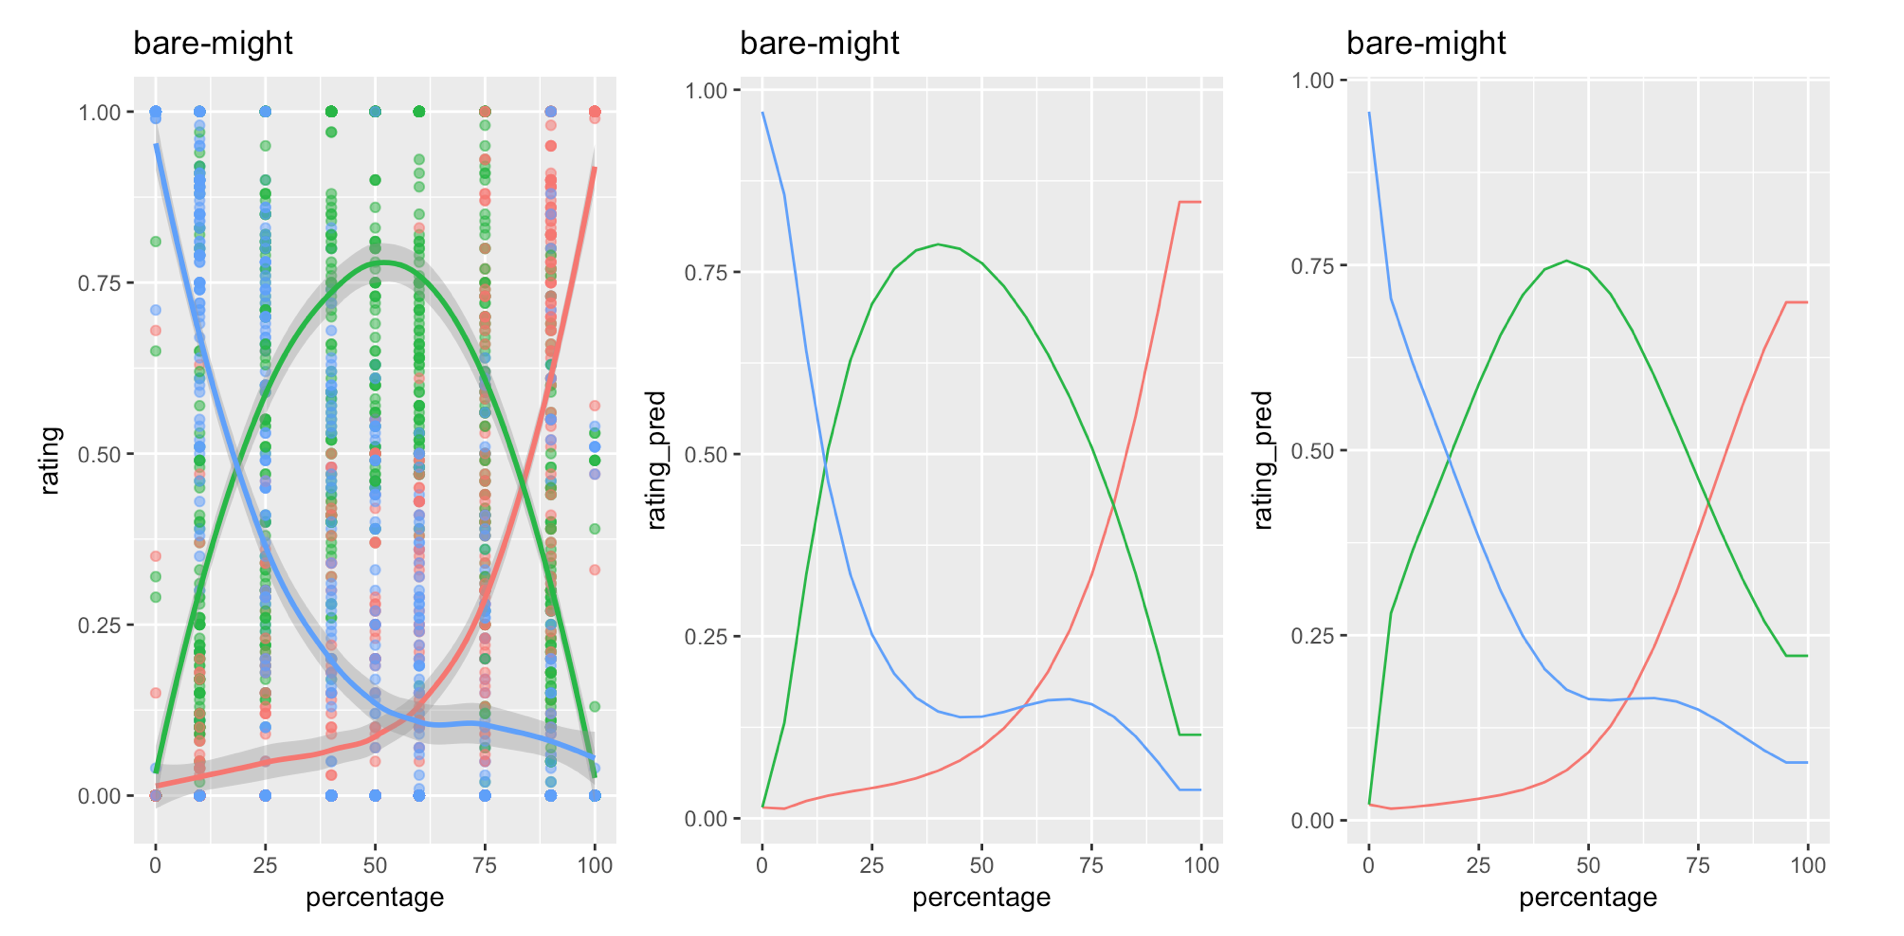
\includegraphics[width=\textwidth]{plots/bare-might-predictions.png} \\
%bare (red) - might (green) condition
%
%\vspace{2em}
%
%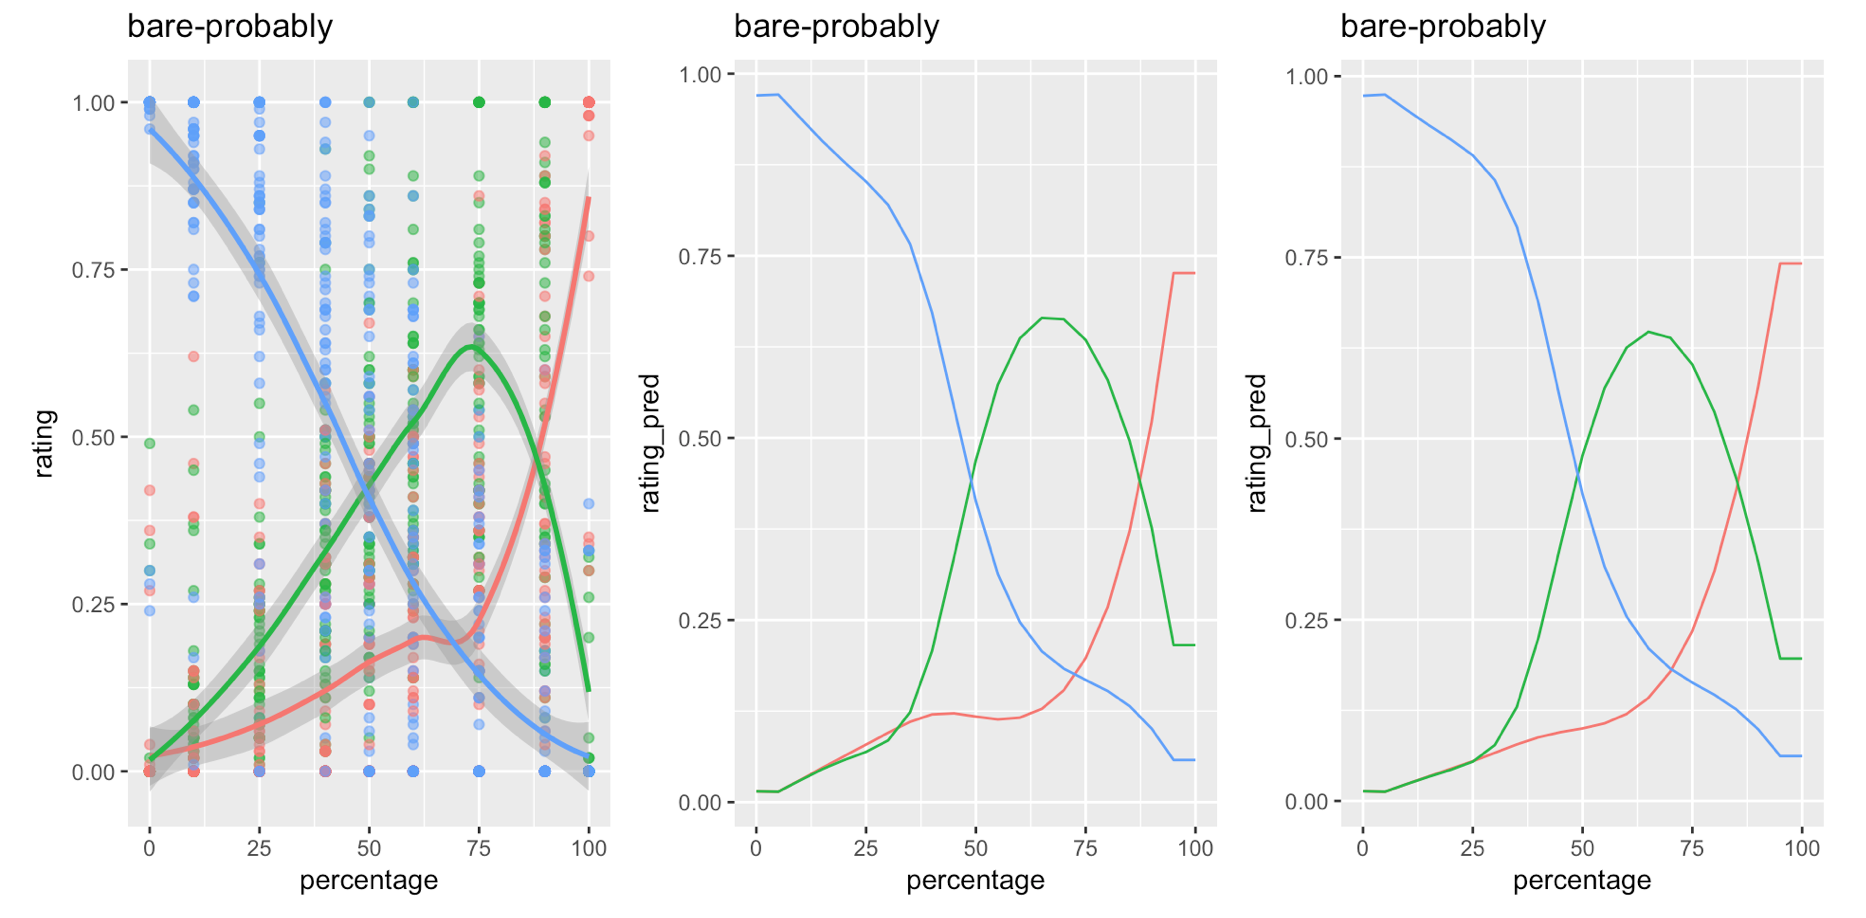
\includegraphics[width=\textwidth]{plots/bare-probably-predictions.png} \\
%bare (red) - probably (green) condition
%
%\vspace{2em}
%
%
%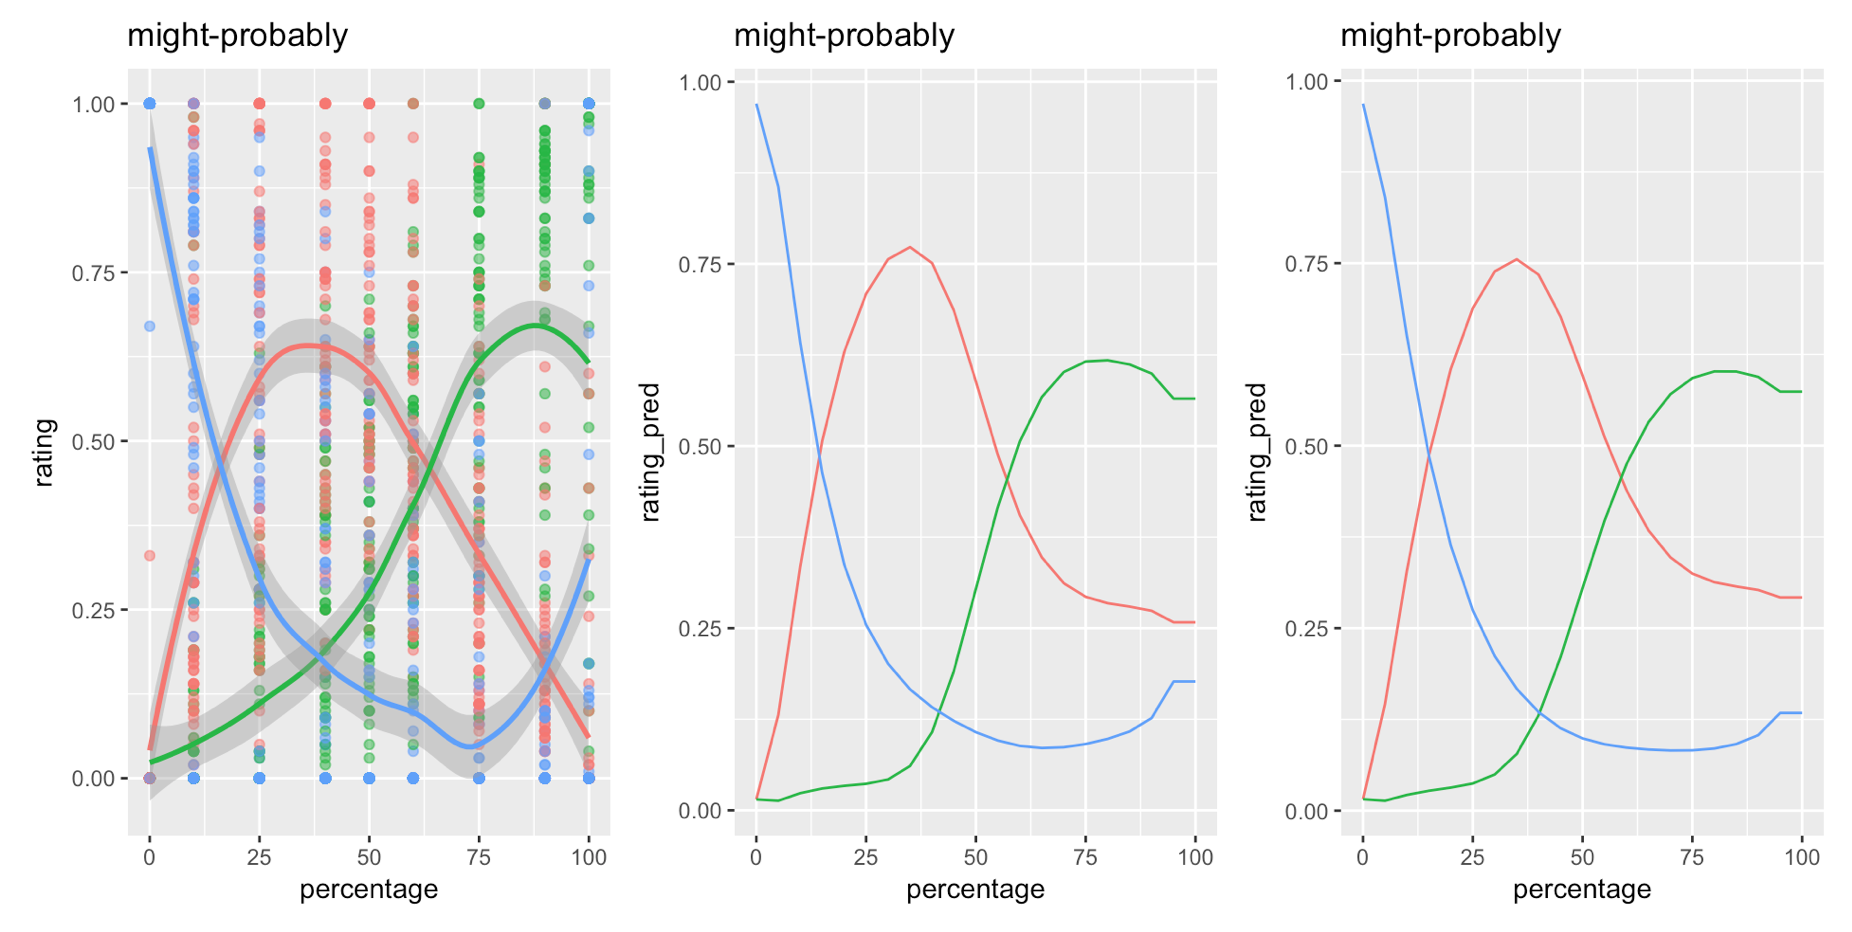
\includegraphics[width=\textwidth]{plots/might-probably-predictions.png}
%
%might (red) - probably (green) condition
%
%\vspace{2em}
%
%
%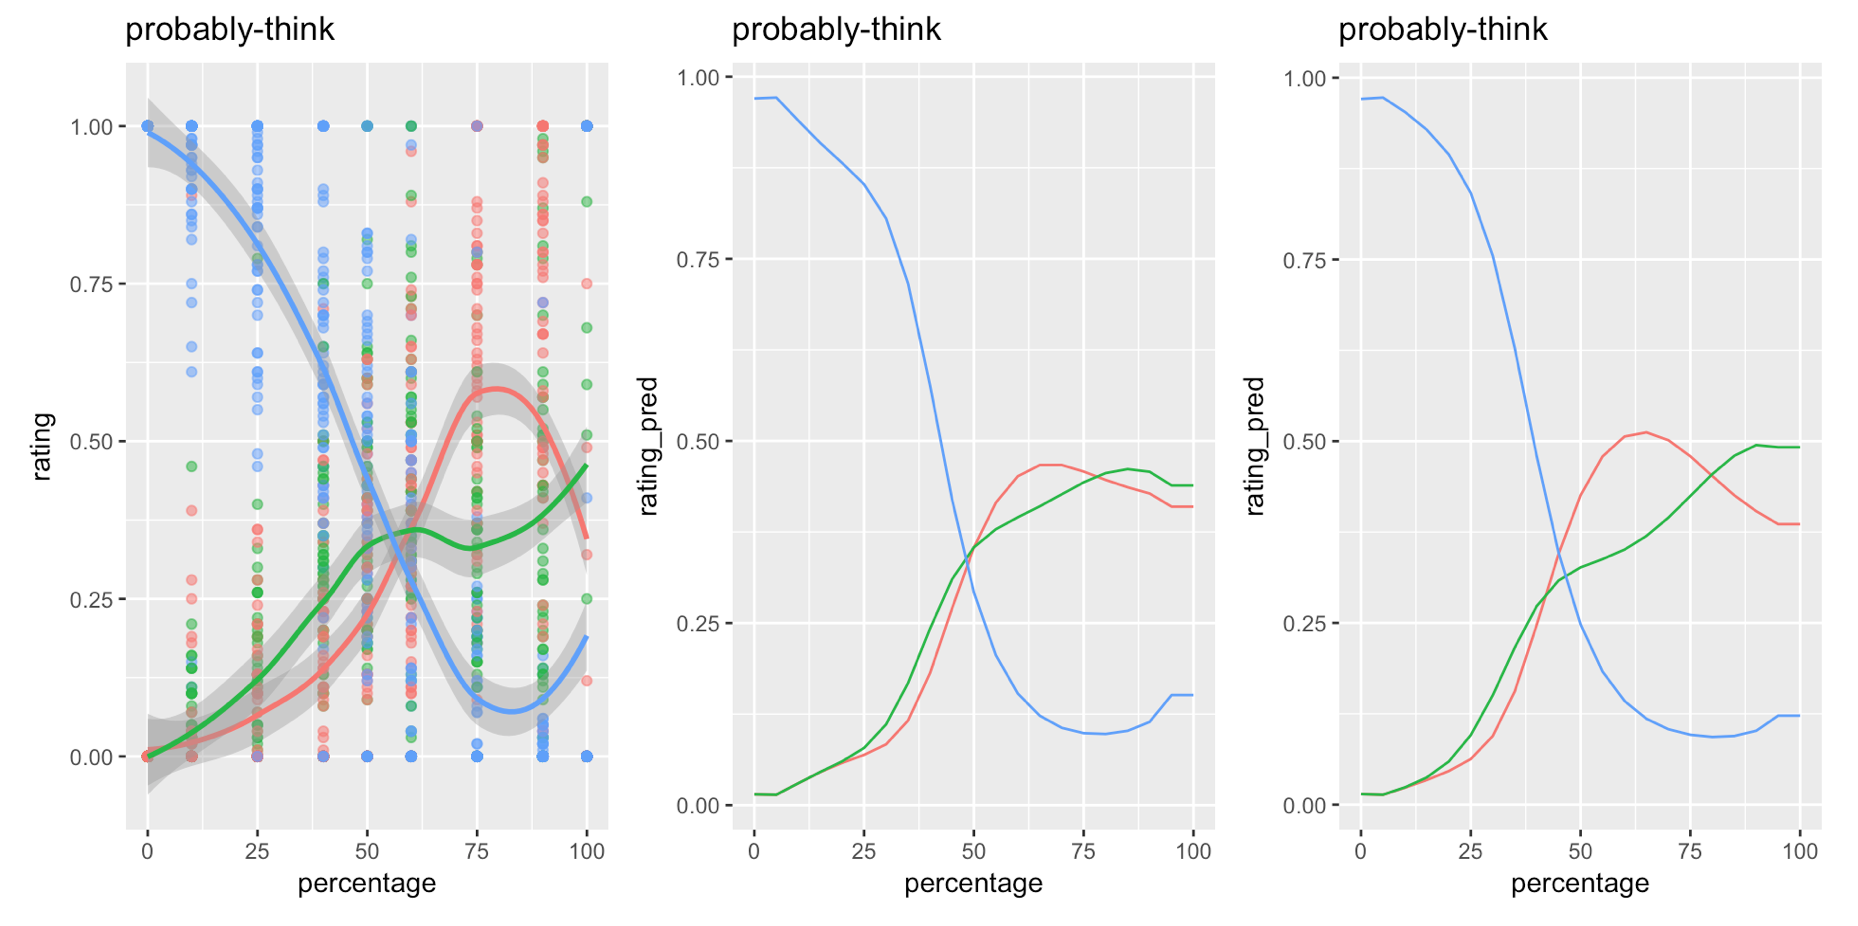
\includegraphics[width=\textwidth]{plots/probably-think-predictions.png}
%
%probably (red) - think (green) condition
%
%\vspace{2em}
%
%
%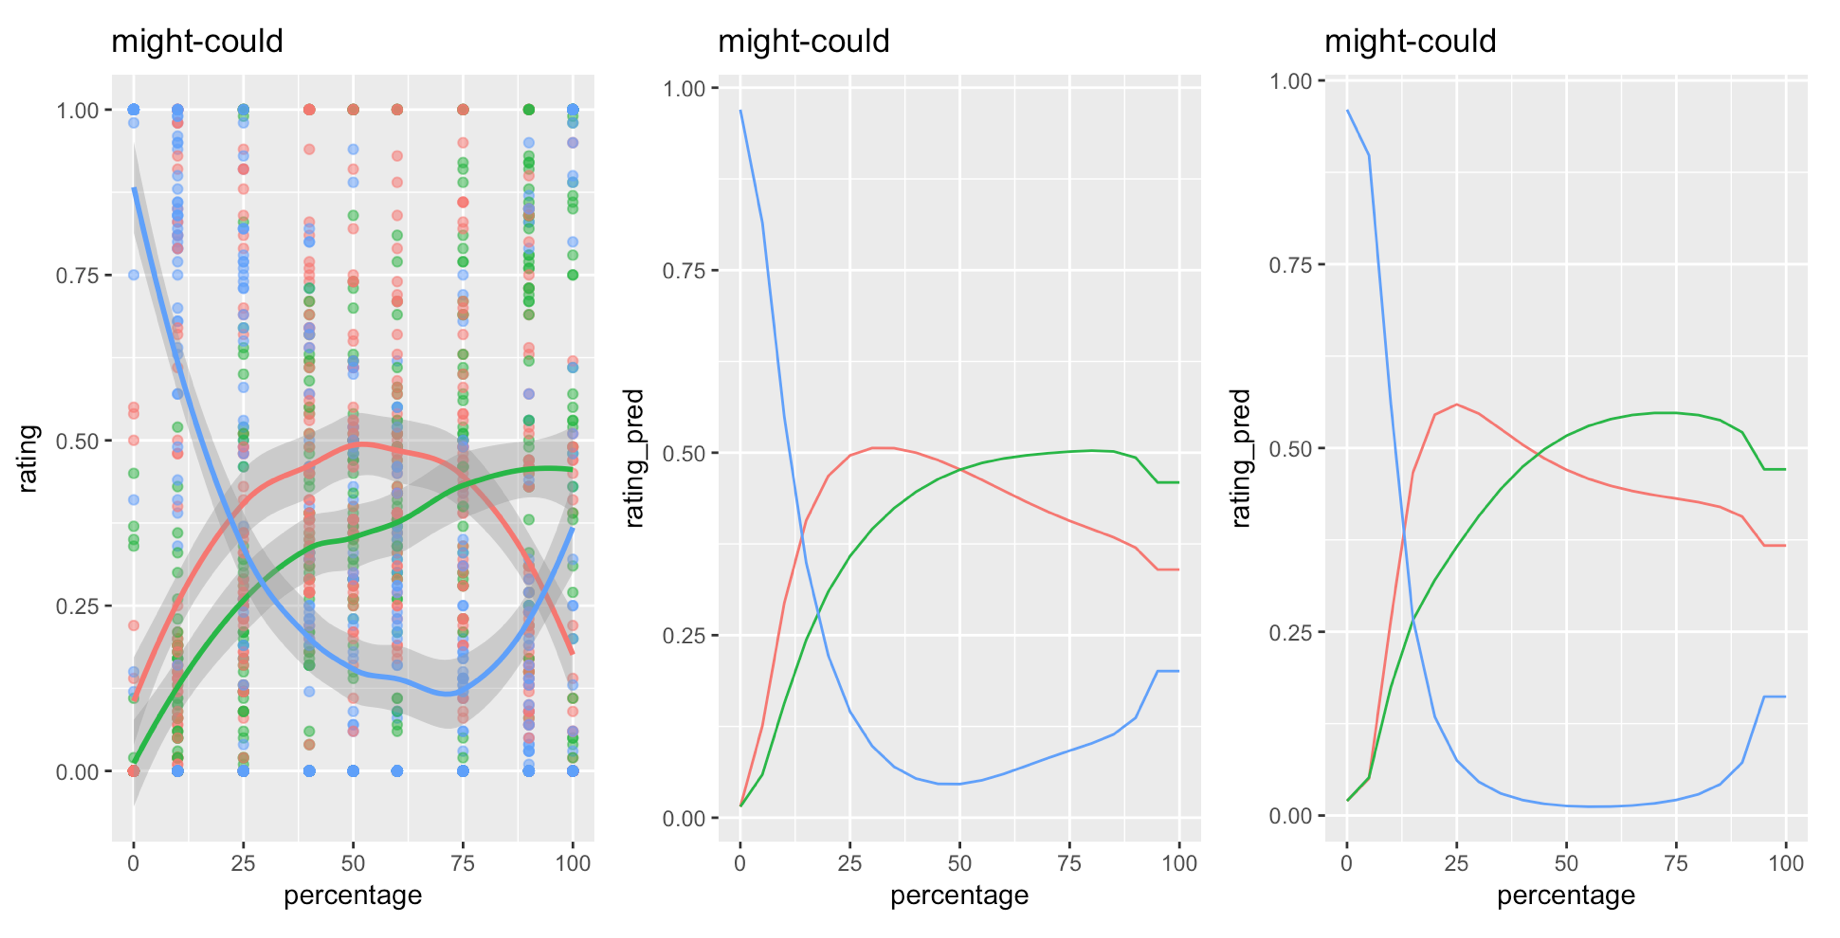
\includegraphics[width=\textwidth]{plots/might-could-predictions.png}
%
%might (red) - could (green) condition
%
%\vspace{2em}
%
%
%\end{center}
%
%In general, the model predicts the average participant responses very well -- in particular in cases in which there are clear contrasts between the utterances (e.g., here in the bare-might, bare-probably, and might-probably conditions). When the two utterances can be used for similar probability ranges (e.g., in the probably-think and the might-could condition), the model deviates a bit more from the experimental data (presumably because there are no clear differences between these two utterances in this context). A second issue with the model seems to be that in some conditions, participants seem to be more rational than the model estimates would suggest. For example, in the might-probably condition, the empirical ratings for \textit{probably} are higher than the predicted ratings.
%
%We also validated our model through cross-validation. In the above figures, the right-most plot shows the model predictions if we estimate model parameters on all conditions except for the one that we are predicting. For example, the right plot for the bare-might condition shows the predictions for this condition if we estimate the parameters using the experimental data from the 14 other conditions. Overall, the predictions with the held-out training data are almost as good as the predictions of the model trained on all the data, which suggests that this is reasonable model for predicting participant's behavior.
%
%One of the advantages of explicitly modeling participants' behavior as a Bayesian model is that we can also inspect the individual parameters, such as the distributions over thresholds $P(\theta_u)$. The following six plots show the estimated $P(\theta_u)$ for the six utterances that we included in our experiments.
%
%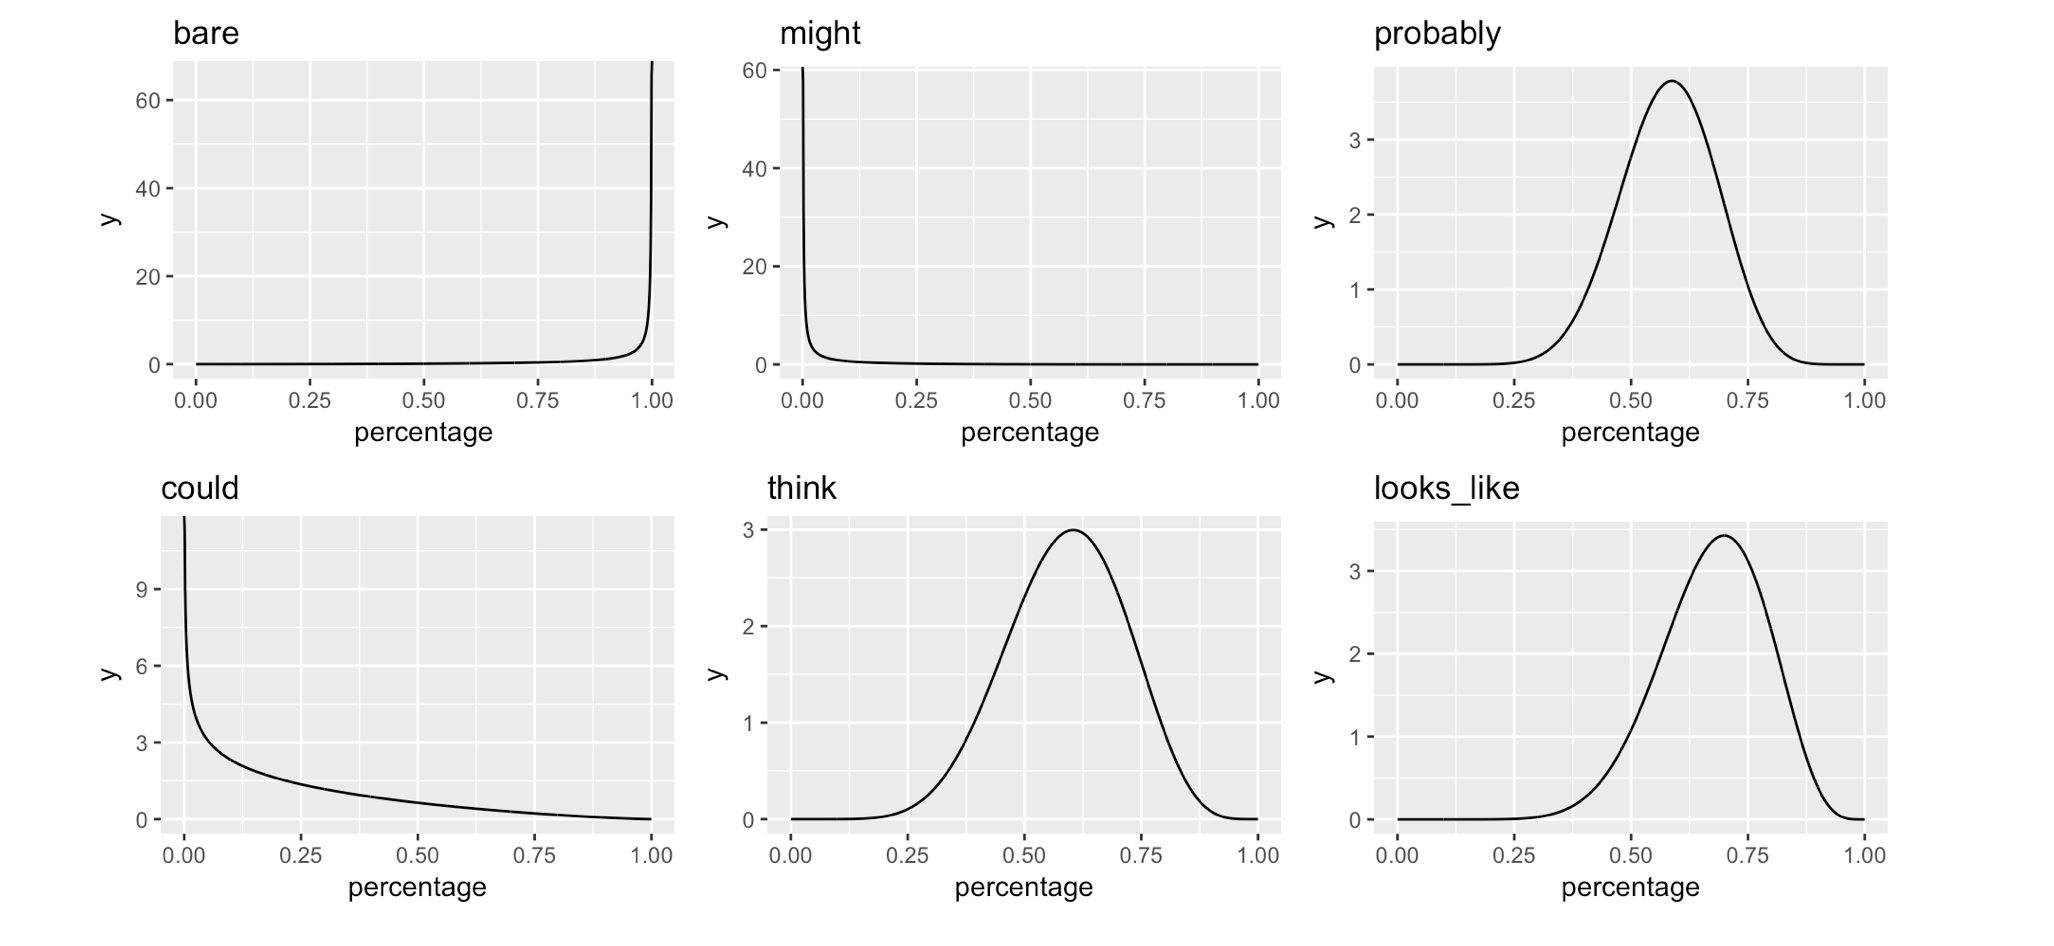
\includegraphics[width=\textwidth]{plots/threshold-distrs.png}
%
%\vspace{2em}
%
%Qualitatively, these estimated distributions are very much in line with semantic theories of modals (e.g., Kratzer (1991)): The  distributions for the thresholds for the possibility  modals \textit{might} and \textit{could} assign most of the probability mass to values slightly above 0; for bare statements most of the probability mass is close to 1 and for \textit{probably}, most of the probability mass is slightly above 0.5. The other two expressions, \textit{think} and \textit{looks like}, have--at least in this context--similar meanings as \textit{probably}. Furthermore, these results are also in line with recent experimental results by Pogue and Tanenhaus (submitted), who explicitly asked participants to rate how much certainty a speaker using these expressions conveyed.
%
%
%
%
%\subsection{Adaptation model}
%
%\subsubsection{Model and estimation}
%
%We model the adaptation process as participants  a) gaining certainty about the threshold distribution that a speaker uses and b) updating the cost parameters for the individual utterances. Our main interest is in how participants update their beliefs about the thresholds for a given speaker but considering that the speaker in the exposure trials only uses \textit{might}, \textit{probably} and bare utterances, the exposure phase also suggests to participants that the speaker has a preference for these utterances over other utterances, which we can explicitly model by allowing the adaptation model to change the cost terms for different utterances. For the exposure phase, we assume that the cost of an utterance is always $c_u$ because are not presented with alternative utterances.
%
%\vspace{1em}
%
%\textbf{Q:} Is this a reasonable argument for/the right way of changing the cost structure during the exposure phase?
%
%\vspace{1em}
%
%
%We assume that participants are doing Bayesian belief updates when they observe utterances during the exposure trials (similarly as Qing (2014) for his model of quantifier adaptation).
%
%\begin{align*}
%P(\theta, c \mid \mathscr{D}) &\propto P(\theta, c) P(\mathscr{D} \mid c, \theta)  \\
%& = P(\theta, c) \prod_{d \in \mathscr{D}} P_S(u_d \mid \phi_d; c, \theta)
%\end{align*}
%
%For the priors over thresholds $P(\theta_u)$, we take the priors that we estimated from the pre-test experimental data. For the costs, we sample from a normal distribution with $\mu=c_u$ (also estimated from the pre-test experimental data) and $\sigma=2$. The data  $\mathscr{D}$ are the 20 utterances that participants hear during the exposure phase. 
%
%\subsubsection{Model predictions}
%
%
%Participants performed the same task as in the \textit{might-probably} condition of the pre-test experiment after the exposure phase. We use the same model as in the pre-test experiment to predict participants' ratings for the utterances \textit{might} and \textit{probably} except that we are using the updated cost parameters and priors over thresholds. We use the same cost function as in the pre-test experiment, i.e., we assume that the cost for the two given utterances \textit{might} and \textit{probably} is 0.
%
%The following plots compare the post-exposure experimental results to the predicted ratings of the model for the two adaptation conditions.
%
%
%\begin{center}
%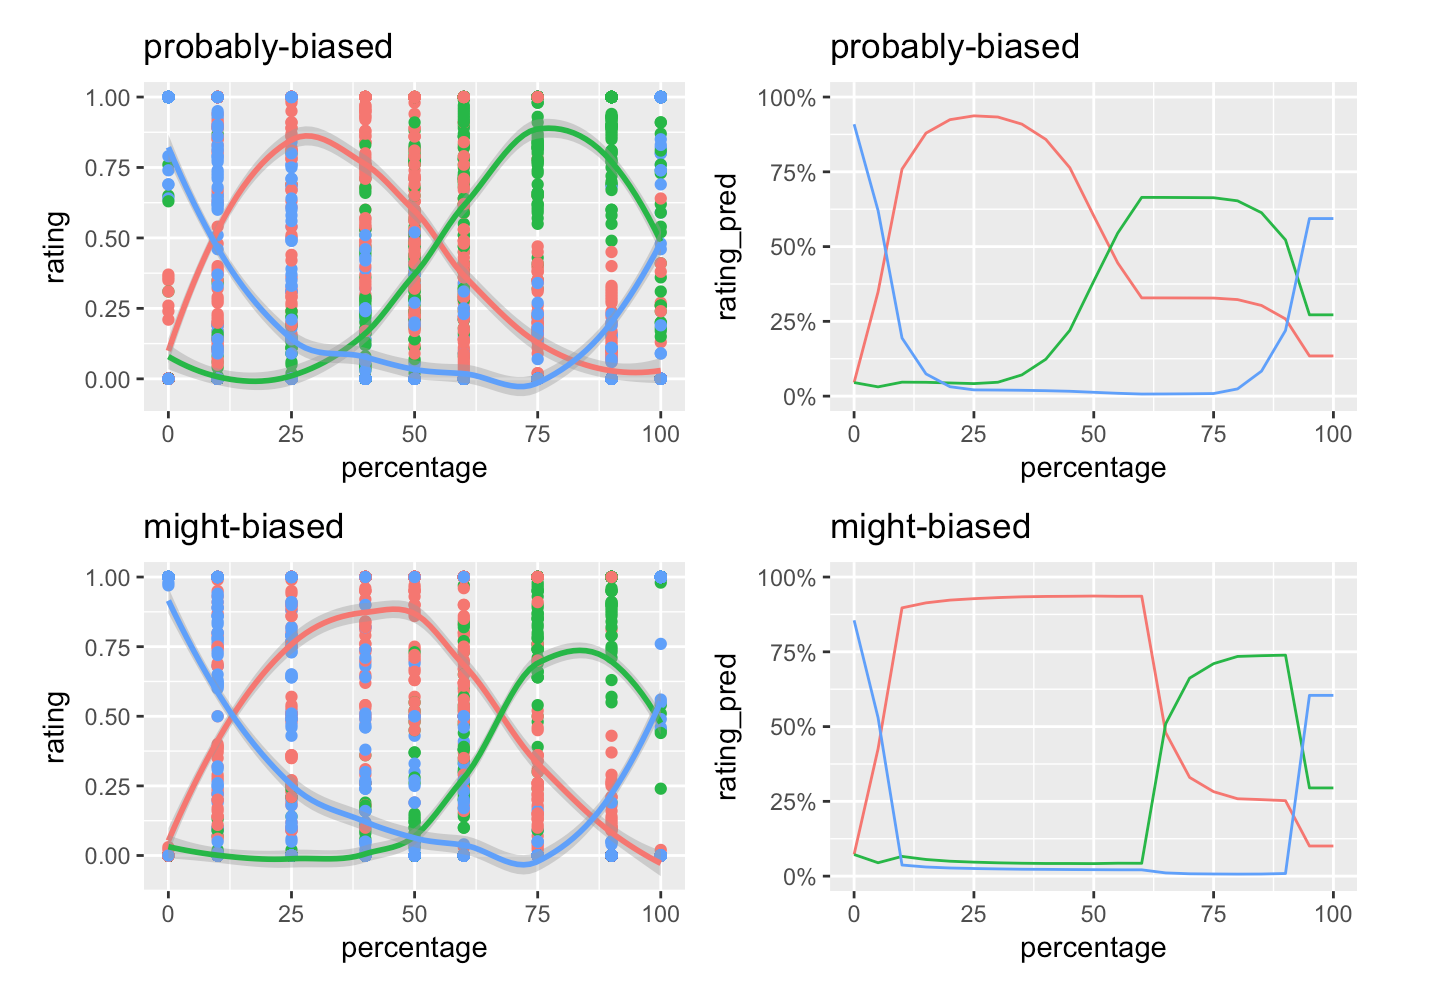
\includegraphics[width=\textwidth]{plots/adaptation-results.png}
%
%Experimental and predicted ratings for might (red), probably (green) and other (blue) for participants in the two adaptation conditions.
%
%\vspace{2em}
%\end{center}
%
%As these figures show, the model matches more or less the experimental results. In the probably-biased condition the model predicts that the curves cross at around 55\% of blue gumballs, which is what we observed in the data and similarly, the predicted and the actual point of intersection of the two curves in the might-biased condition are at around 65\%. However, the issue of too low ratings for \textit{probably} and the bare utterances that we already observed in the pre-test experiment, seems to be even stronger here. This effect could be lowered by increasing the rationality parameter $\lambda$ but it is not clear why people would be more rational in the adaptation experiment than they were in the pre-test experiment.
%
%Alternatively, we could consider using a different literal listener which does not assign a uniform probability to all event probabilities $\phi$ if they are above $\theta_u$. But again, it is unclear what these distributions would look like.
%
%As in the pre-test experiment, we can again look at the posterior distribution of $P(\theta)$ and the cost parameters for the two conditions.
%
%
%\begin{center}
%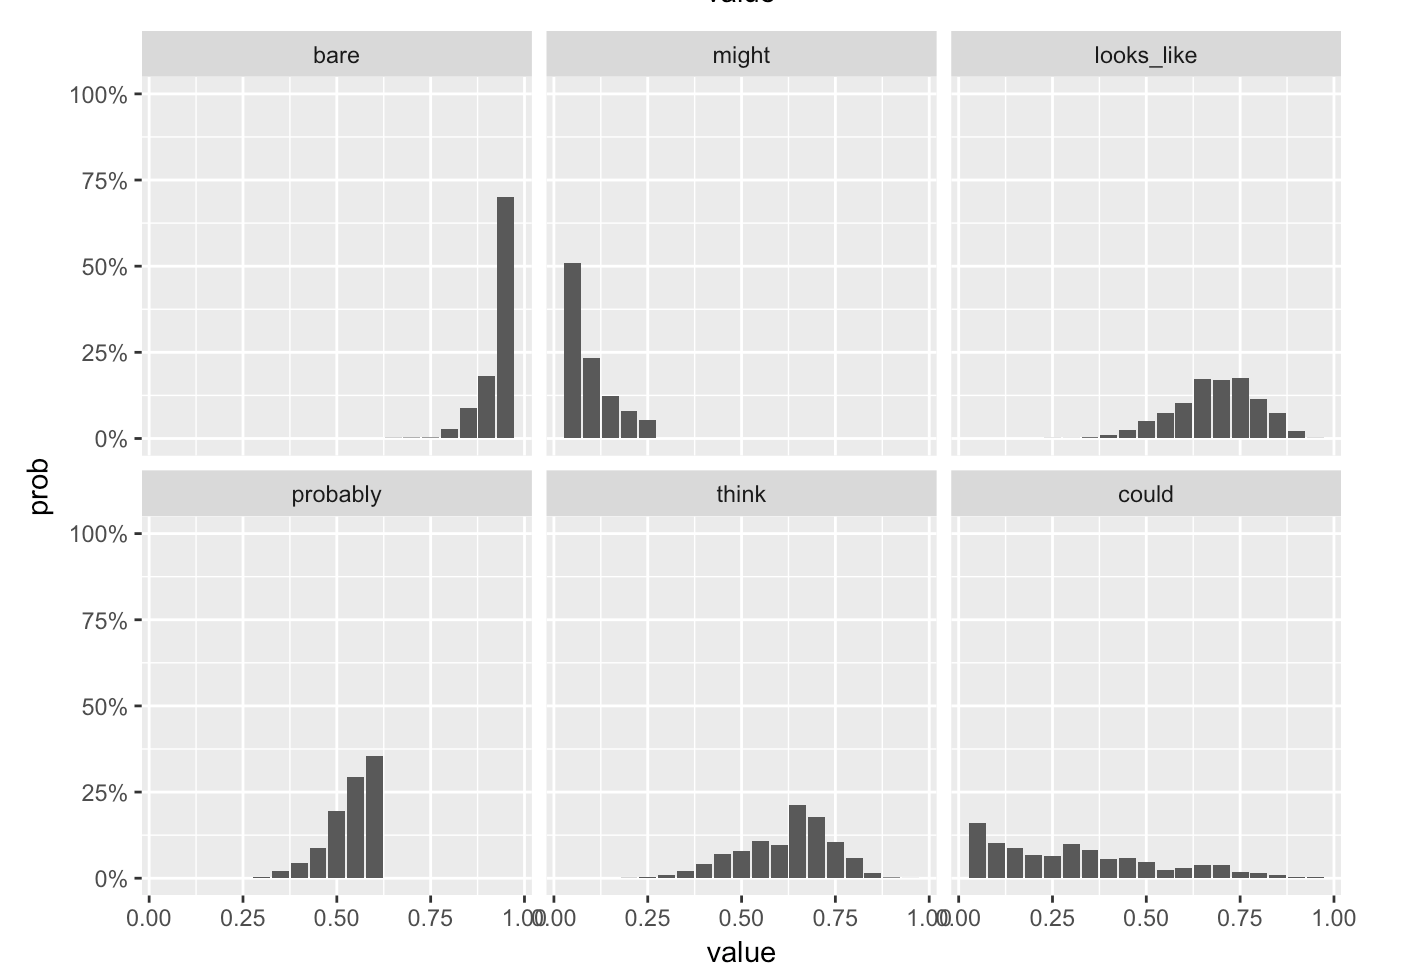
\includegraphics[width=0.9\textwidth]{plots/probably-biased-threshold-posterior.png}
%
%Posterior distributions over threshold parameters $\theta$ in the \textbf{probably-biased} condition.
%\end{center}
%
%\begin{center}
%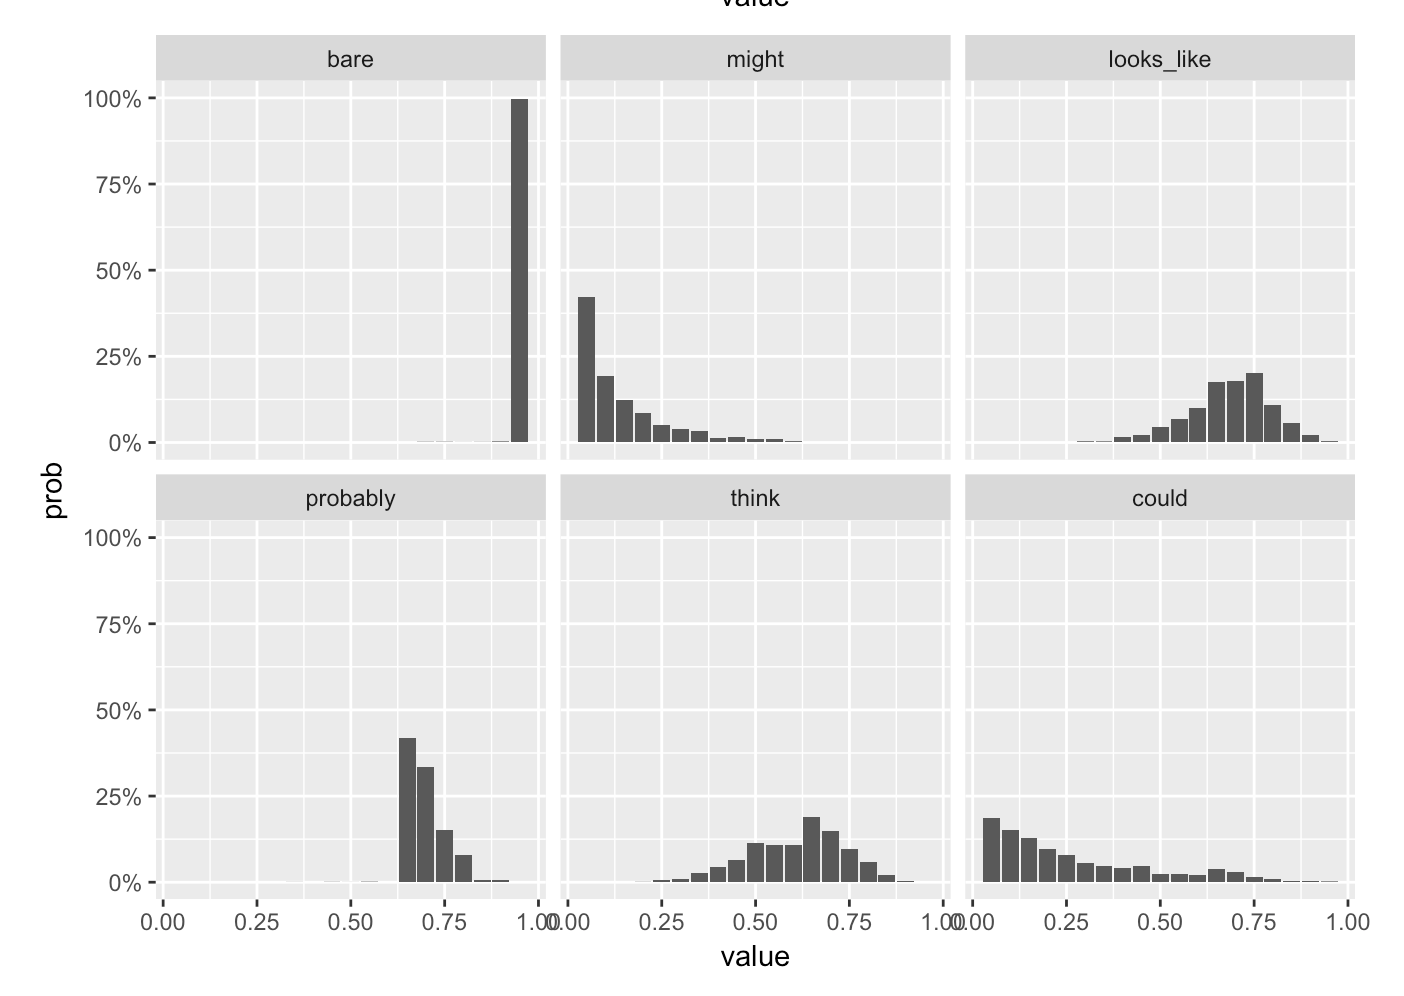
\includegraphics[width=0.9\textwidth]{plots/might-biased-threshold-posterior.png}
%
%Posterior distributions over threshold parameters $\theta$ in the \textbf{might-biased} condition.
%\vspace{2em}
%\end{center}
%
%These plots suggest that the distributions over thresholds for the three utterances that do not appear in the exposure phase remain fairly broad and match to a large extent the prior distributions.
%This suggests that participants are not updating their beliefs about the use of these expressions, which is expected given that they do not see any evidence for the use of these expressions. 
%
%\vspace{1em}
%\textbf{Note:} Would be interesting to collect post-exposure ratings for e.g., the pair \textit{could} and \textit{looks like} and see if these things remain more or less unchanged.
%\vspace{1em}
%
%The distributions over thresholds for bare utterances, \textit{might} and \textit{probably}, on the other hand, differ considerably across the two conditions and are overall much narrower. In the \textit{probably-biased} condition, 
%the model infers that the threshold should be at or slightly below 60\%, and the threshold for \textit{might} should be somewhere between 5 and 25\%.
%
%In the \textit{might-biased} condition, the distribution of $\theta_{might}$ has a slightly longer tail but overall still assumes that the threshold is low.  The distribution of $\theta_{probably}$ in this condition, is shifted to the right with the most likely threshold being at 65\% and given that the speaker in this condition always uses \textit{probably} to refer to events which are 90\% likely to happen, the distribution for $\theta_{bare}$ is also shifted to the right and much narrower. 
%
%Overall, these thresholds seem very reasonable and what is noteworthy is that the model still assigns a high probability to utterances with \textit{might} to describe events whose probability of happening is low despite the fact that participants only observe \textit{might} being used to describe  events with a probability of happening of 60\%.


%\section{Future directions/TODOs}
%
%{\bf Short-term things:}
%
%\begin{itemize}
%\item The bootstrapping procedure to estimate the variance of all $\Theta_S$ parameters potentially leads to too high estimates for the variance. One should try to turn this into a hierarchical model which puts a prior on the overall variance.
%\item We assume right now that the comprehension model should be an $L_1$ and the production model should be an $S_1$. One could also imagine that the production model should be an $S_2$. Investigate this hypothesis (in particular in light of the newly collected comprehension norming study.)
%\item Try estimating the means and variance of the hierarchical model for the Beta distributions using the mean and $nu$ parameterization -- potentially more stable than $\alpha/\beta$ parameterization.
%\item Run experiment with equal number of {\sc might} and {\sc probably} utterances to rule out only priming.
%\item Figure out if there is a way to include an ``adaptation rate''  parameter, similar to Roettger and Franke (unpublished)
%\item Try to investigate whether it's actually linguistic adaptation or rather inference of some higher-level goal (e.g., not wanting to upset the girl).
%\end{itemize}
%
%{\bf Long-term things:}
%\begin{itemize}
%\item Run experiments with multiple speakers.
%\item Run post-exposure phase with utterances that were not part in exposure (e.g., \emph{could}, \emph{looks like}). What changes about these? What does the model predict?
%\item Run experiment where the speaker uses semantically very similar items (e.g., \emph{probably} and \emph{think}) differently. Do participants also learn these differences?
%\item Run norming study  -- exposure -- prior elicitation -- production post-exposure -- comprehension post-exposure -- to verify model on individual participant level.
%\item Implement hierarchical model which can explain adaptation to multiple speakers.
%\item Consider adaptation to speakers with accents -- one potential way to model this would be to model these speakers as having more noise. This would predict that people rely more on their priors and adapt slower. (Also compare this to Gibson et al. (2017).)
%\item Consider generalizations of adaptation: Does adapting to one female speaker skew expectations more to other female speaker than to other male speaker? And vice versa? What about accents? Is this at all a function of similarity in speech (e.g., as discussed in Kraljic (2015) or Johnson (2006)).
%\item come up with paradigm where people only get indirect feedback (i.e, did something happen or not, maybe some betting game).
%
%\end{itemize}



\end{document}
